\documentclass{article} % For LaTeX2e
\usepackage{nips12submit_e,times, color, amsmath}
\usepackage{natbib}
\usepackage[pdftex]{graphicx}
\usepackage{subfigure}
%\documentstyle[nips12submit_09,times,art10]{article} % For LaTeX 2.09


\title{Binary Separation on Heterogeneous Image}

\author{
Fisher Yu \\
\texttt{fy@princeton.edu}
\And
Nanxi Kang \\
\texttt{nkang@princeton.edu} 
\And
Siyu Liu\\
\texttt{siyuliu@princeton.edu}
}

\newcommand{\fix}{\marginpar{FIX}}
\newcommand{\new}{\marginpar{NEW}}

\nipsfinalcopy % Uncomment for camera-ready version

\begin{document}

\maketitle

%test citation~\citep{Boykov2006graph}

\section{Introduction}

%\subsection{Background}

In computer vision, ``Image Segmentation'' is a process of partitioning an
image into several pixel groups. It is typically used to locate
objects and boundaries in an image. Particularly, ``Binary Separation'' -
how to partition an image into two segments: ``foreground''
 and ``background'' is of special interest. 

Earlier techniques are either based on boundary features
~\citep{Kass1988snakes} or manual sketches
~\citep{Boykov2006graph}. In this project, we propose a new
approach to partition ``foreground'' and ``background'' making use of 
distance data of real objects in the image. To be specific, when an
image is taken by camera, there exists a
one-to-one mapping from pixels in the image to real objects. 
For each image to be processed, we have additional data telling the 
distances between the camera and the real objects corresponding to some
 pixels in the image. 

It is challenging to use the distance data. Although the distance data
is helpful, yet it is not complete. A typical distance data set only
covers approximately 10\% pixels.It is necessary to develop techniques
that infers the states of other pixels based on this sparse
information. Besides, the data could contain some errors. For example,
some pixel may be mapped to a wrong real object resulting in a wrong
distance number. Therefore, the algorithm should include procedures
that help fix the inherent errors of data. 

Considering the defects of distance data, we plan to only use it to
generate the initial states of pixels, i.e,
 whether it belongs to ``foreground'' or not. Based on the inital
 states, we'll iteratively refine the segmentation following the
 traditional Expectation Maximization process. To do the refinement,
 we'll use Markov Random Fields to calculate the log-likelihood of a
 pixel, taking the information of the 8 pixels around it into account.

We believe our approach is more accurate than previous work. The additional 
distance data is a good indicator about which group a pixel belongs to, 
thus giving us confidence in the accuracy of segmentation, compared to earlier
 techniques which only use the image information alone. Moreover, our
 approach is flexible in that it does not need manual annotation. Finally, the
segmentation decision is not likely to be misled by errors in distance
data, since it will do iterative refinement based on the pixel's local
neighbor information.

\section{Related Work}
As a common problem in computer vision, segmentation has been well
studied in the past. There is a large literature on segmentation and
clustering, among which two main lines of methods are proposed
previously, feature space clustering
(e.g.~\citep{Comaniciu1997featurespace},~\citep{Comaniciu1999meanshift})
and graph-based approach
(e.g.~\citep{Shi1997normalizedcuts},~\citep{Wu1993optimalgraph}).
Besides these methods, which only relies on the image
information , researchers have proposed new segmentation algorithm
that use rough manual labelling to do more accurate segmentation. We
will introduce these three methods briefly.


In feature space clustering, local features, such as low pass filter
response, SIFT~\citep{Lowe2004sift}, etc., are firstly extracted from
the given image. For color images, color information is often
included. Then those features are concatenated to form a vector as a
descriptor for each pixel. In order to segment the image, we might
seek a clustering of feature vectors observed in the image. A compact
region of image with distinct feature would be expected to have a
corresponding high density area in the feature
space~\citep{Boykov2006graph}. 


% A natural approach is to model the observed feature vector using a
% Gaussian mixture model (GMM)~\citep{Carson2002bolbworld}. For a
% pre-determined number of clusters \textit{K}, the parameters can be
% fitted by Maximum Likelihood using EM algorithm. In addition,
% \textit{K} can be chosen using penalized likelihood (a.k.a. minimum
% description length), Baysian information criterion (BIC) and other
% model selection mechanisms. In addition, other variations are proposed
% by replacing GMM with K-means or low dimensional representation of the
% covariance matrix via matrix factorization. On the other hand, to
% avoid extra step of determining the number of clusters for the methods
% mentioned above, a non-parametric model based on kernel density
% estimation is proposed as an alternative. Mean-shift segmentation
% algorithm~\citep{Comaniciu2002robustapproach} considers the
% probability density of feature vectors obtained from a given image. An
% iterative update on the mean-shift equation is used to find the
% segmentation labels. 


Another branch of image segmentation algorithms is graph-based
method. Instead of consider each pixel independently, we form a graph
with each vertex representing an individual pixel and assign weights
to edges according to some similarity measure. Then, the segments are
determined by graph cuts.


%One naive approach would be to calcualte connected components. We could use algorithms like Kruskal or Prime to simple remove edges between dissimilar pixels. However, this method is not robust to stray links. Thus,~\citet{Felzenszwalb2004Efficient} introduced an improved version of Kruskal algorithm which takes in account the local variantion within each component. An alternative proposal is to formulate segmentation as a max-flow/min-cut problem. One typical example of S-T Min Cut algorithms is the normalized cut introduced by~\citet{Shi2000Normalized}. This method takes into account the partition size of each segment so as to avoid tiny regions. In a more sophesticated setting, Markov Random Field (MRF), which we chose a variant version, Conditional Random Field (CRF), for this project, is often used to combine probabilistic modeling and graph cut in order to provide better result. The goal of learning MRFs is to minimize the objective function (a.k.a. the energy function) which describes both fitness and connectivity among neighborhood. Several training algorithms have been proposed over the years, Iterated Conditional Modes (ICM)~\citep{Besag1986statisticalanalysis} uses "greedy" strategy to find local minimum; Graph Cuts, two most popular ones, swap-move and expansion-move were introduced in~\citet{Boykov2001Fast}; Max-Product Loopy Belif Propagation (LBP)~\citep{Felzenszwalb2004Efficient} and~\citep{Freeman2000lowlevel}, a variant algorithm from the original belif propagation supporting loops in the graph; Tree-reweighted Message Passing desbribed in~\citet{Kolmogorov2006messagepassing}.


A recent new approach 
by~\citet{Boykov2006graph} relies on manual sketches on the original
 image. It requires a user to draw strokes of different color in the foreground 
and background area of the image. Then, the algorithm solves segmentation
problem based on this extra knowledge. 

\section{Data}

We got our data from Google street view team and preprocessed it for
use in our project. The data was collected by a car equiped
with 8 cameras and 3 laser scanners. Each of the laser scanner can
scan a 180 degree 2D plane at each time. Two of the laser scanners
scanned vertically and the third one scanned horizontally. As the car moved, the car
positions were recorded by global positioning system. Those positions
were adjusted by the scans of the horizontal laser scanner using SLAM
(Simultaneous localization and mapping) techniques to get the best
precision. The 3D position of each laser scan point can be
estimated based on the relative positions of the car and laser
scanners and therefore a 3D point cloud can be built from the scans of
the vertical laser scanners. At the same time, the eight
cameras were taking pictures as the car moved. Although the cameras
were well calibrated, the images were taken by rolling shutters and
there could exist errors in terms of image projection model if we assume each
image were taken in a pinhole model.

Given the 3D point cloud and images, we project the points onto the
images with the estimated point positions, camera poses and projection
matrices. Then we can get images like Figure~\ref{fig-data_image}.

\begin{figure}[h]
\begin{center}
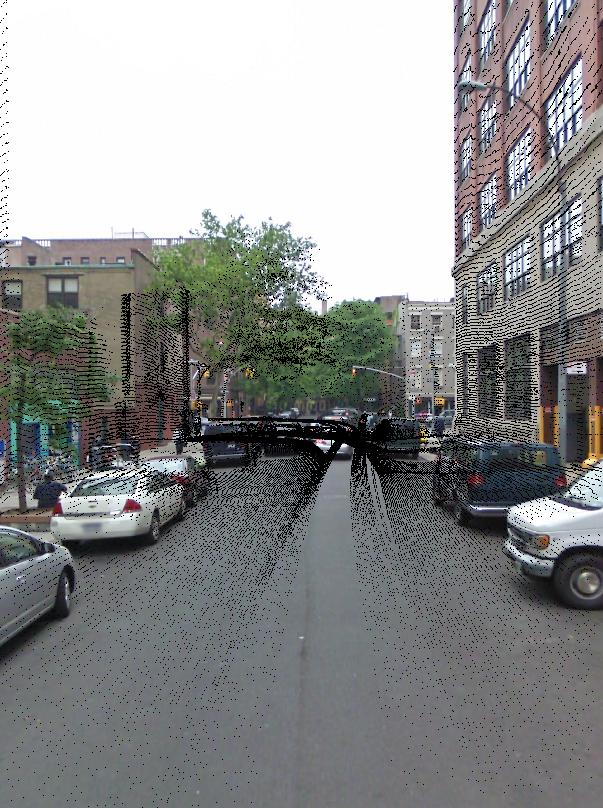
\includegraphics[height=0.5\linewidth]{./fig/overlay_00_00.jpg}
\end{center}
\caption{An image with 3D points projected into it.}
\label{fig-data_image}
\end{figure}

In Figure~\ref{fig-data_image}, the black dots are the projections of
the 3D points on this image. As we can see, due to all kinds of possible
errors mentioned above, the 3D projections and the images are not well
aligned and we can't segment the images directly based on the depth of
the 3D scan points. In this project, we want to find the contour
between the background (the sky area) and foreground (all the objects
appears in the image, including roads and buildings). The models and
computing issue will be discussed in the methods section.



\section{Methods}
Based on the previous work, we merge several ideas in our
project. First, to classify a pixel, we can first train a Gaussian
mixture model to summarize the variation of pixels in the background
and foreground separately. In another way to see this, we are getting
an approximate distance from a certain pixel value to the cluster it
belongs to and therefore we can get a cost to assign a certain pixel
to the foreground or background. On the other hand, in the Gaussian
mixture model, we are assigning an latent variable to each pixel. Due
to the isolation between adjacent pixels in the Gaussian model, it is
easy to imagine that the output of the binary classification will be
very noisy in the sense that the adjacent pixels will have different
labels although they have similar colors and belong to the same object
visually. To solve this problem, we use \emph{Markov Random
  Field}(MRF) model to constraint the relation between the labels of
adjacent pixels. Also, we use conditional random field(CRF) model to
adapt this relation to the difference of the pixel colors and
therefore the model becomes more flexible. Also, we explore various
ways to utilize our laser data. In the following subsections, we will
discuss parts of our model and elaborate how we use the scan data.
\subsection{Gaussian Mixture Model}
The foreground and background shall have different color
characteristics. We use Gaussian Mixture Model to summarize the colors
of background and foreground. We train the two models separately,
which means given a estimate of foreground and background pixels, we
don't change the label of the pixels and only aim to find a more
accurate model to describe the given labels. We use standard EM
algorithm to train the models.
\subsection{Conditional Random Field}
To solve the discontinuity problem in only using distance to the
closest Gaussian mixture model as a cost, as what has been down in the
literature, we add a connection cost between adjacent pixel labels to
encourage identical labeling. Our proposed model is
\begin{align}
\mathbf{E}(\mathbf{c}, \mathbf{d},\mathbf{k}, \mathbf{\theta},
\mathbf{z}) &= U(\mathbf{c},\mathbf{k}, \mathbf{\theta}, \mathbf{z}) +
V(\mathbf{c}, \mathbf{d}, \mathbf{z}) \label{eq:energy}\\
U(\mathbf{c},\mathbf{k}, \mathbf{\theta}, \mathbf{z}) &=
\sum_{i=0}^{i<N} D(c_i, k_i, \theta, z_i) \\
D(c_i, k_i, \theta, z_i) &= -\log \pi_{k_i}^{z_i} + (c_i -
\mu_{k_i}^{z_i})^T (\Sigma_{k_i}^{z_i})^{-1} (c_i - \mu_{k_i}^{z_i})
\\
V(\mathbf{c}, \mathbf{d}, \mathbf{z}) &= \gamma \sum_{(i, j) \in
  \mathcal{N}} [z_i \not = z_j] e^{ -\beta d_i \| c_i - c_j\|^2}
\end{align}
\textbf{c} is the set of pixel colors.
\textbf{d} is  how likely a given pixel is on the boundary from
scan. It will be discussed further later in this section.
\textbf{k} is assigned GMM cluster for each pixel.
\textbf{z} is latent variables labeling foreground and background
where $z=0$ means foreground and $z=1$ background.
$\pi_k^z$ is mixture weighting coefficients.
$\mu_k^z$ is the mean of the $k$th Gaussian component.
$\Sigma_k^z$ is the covariance matrix of the $k$th Gaussian component.
$\gamma$,$\beta$ are parameters to control the connection cost.
$\theta$ is the set of parameters of the Gaussian mixture model and
therefore $\theta$ = \{$\pi$, $\mu$, $\Sigma$\}.
$\mathcal{N}$ is set of all the neighbor pixels and we don't use
diagonal neighbor in the experiments. $N$ is the number of pixels in
the image. $\mathbf{E}$ is the energy function representing the cost function we
are going to minimize. It can be decomposed into two
parts. $\mathbf{U}$ is the cost of unary term. As discussed in the
last subsection, it is the Mahalanobis distance to the closest
Gaussian cluster of its labeled Gaussian mixture model, adjusted by
the mixture weighting coefficient of that cluster. Note that we didn't
use soft assigned cluster in the model, as was done commonly in
Gaussian mixture model.~\citet{Rother2004GrabCut} said that in their
experiment, the soft assignment doesn't improve the results greatly
but will make the optimization harder. $\mathbf{V}$ is the connection
cost between adjacent pixels. The cost is adjusted by the additional
information including the pixel color difference and the scan
information. The idea is that if the color difference is large or the
pixels are likely on the boundary of different segmentations, the
inconsistent labeling cost will be small. Otherwise, if two adjacent
pixels have very similar colors, they are more likely to have the same
labeling. In our case, we consider the color image instead of gray
image and so the different difference of pixel colors are measured by
L2 norm.

It can be shown~\citep{Geman1984Stochastic, Li2001Markov} that the
energy function we defined to represent the CRF corresponds to a
Gibbs distribution uniquely. So by minimizing the energy function, we
are actually seeking the Maximum Likelihood solution to the Gibbs
distribution. The graphical representation of our model in color is
shown in Figure~\ref{fig:mrf_model}.

\begin{figure}[h]
\begin{center}
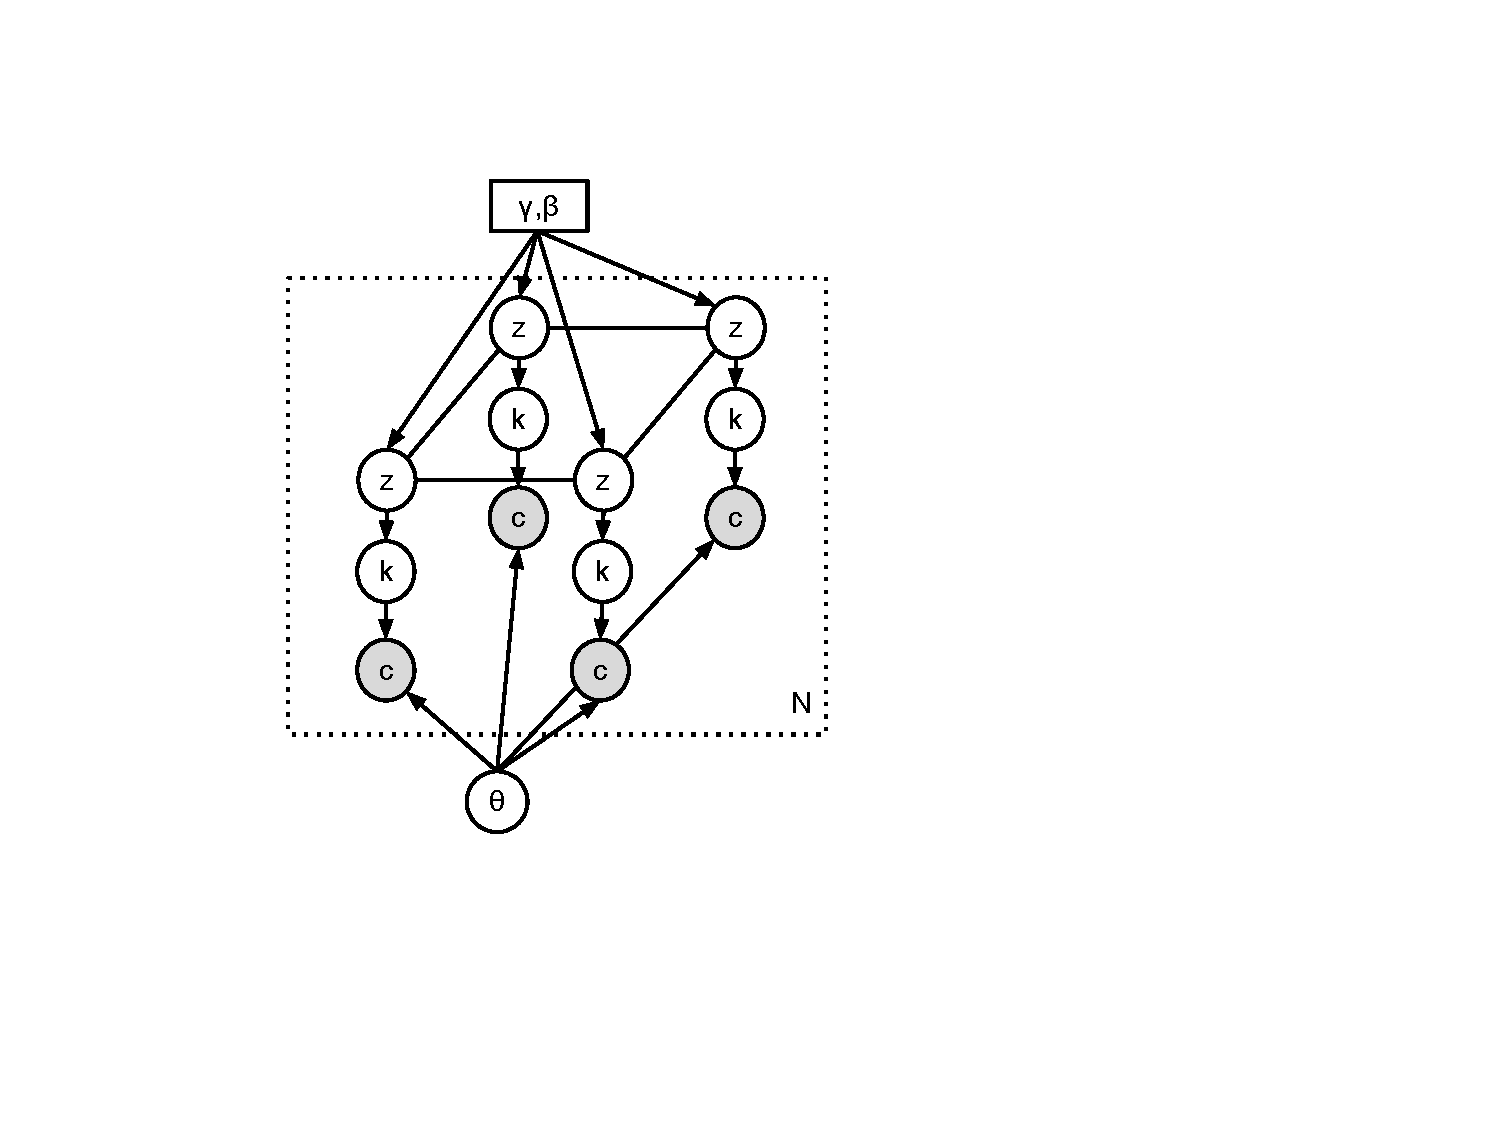
\includegraphics[height=0.5\linewidth]{./fig/mrf_model.pdf}
\end{center}
\caption{The graphical representation of our model in color}
\label{fig:mrf_model}
\end{figure}

It is worth pointing out that when \textbf{d} is always 1. The model is
called GrabCut as in~\citep{Rother2004GrabCut}. When $\beta$ is 0,
which means the inconsistent cost between adjacent pixels is constant,
the model is called Ising model. We have done experiments on those
models and the results are shown in Section~\ref{sec:exp}.

\subsection{Inference}
As mentioned, we use EM algorithm to estimate the Gaussian mixtures in
given the pixel labels. At the end of each iteration, we minimize the
energy function~\eqref{eq:energy} to update the pixel labels. There
are several ways to infer the labels of pixels based on our model. The
traditional way is Monte Carlo Markov Chain
method~\citep{Bishop2006Pattern}. There are also some other inference
methods proposed during the last several
decades~\citep{Szeliski2008Comparative}. However, most of them are
approximate methods and don't guarantee an globally optimal
solution.~\citet{Boykov2001Fast} and~\citet{Boykov2006} argues that for the binary
segmentation, if the energy function has the submodular property, the
optimal solution can be got by minimum graph cut. Fortunately, when we
constructing our energy function, we make sure that the submodular
property is satisfied. Therefore, we solve Maximum flow, the dual
problem of minimum cut, to minimize the energy function and update the
pixel labels at the end of each EM iteration.
\subsection{Use of Scan Data}

As you can see in Figure~\ref{fig-data_image}, the scan points are not
scattered in the image evenly in the foreground and therefore it is
hard to extract some robust statistics to describe the foreground or
the boundary. One idea is using bins around a pixel to describe its
feature. To be specific, given the position of a pixel, we 
consider all the scan points within certain radius. The circle is then
divided in angular direction to get the bins. The feature value of the
pixel is how many pizza shape bins contain scan points. Although it is
a nice way to describe the scan point description around a pixel, it
is hard to find efficient way to calculate it for every
pixel.

We later realized that using bins is equivalent to downsampling the
image. What's more, the region of most interest is the boundary
between the foreground and background. Therefore, we propose a new
methods to extract the scan information from the scan points. First,
we downsample the image and then apply Sobel
filter~\citep{Szeliski2010} to extract the edge-like features. The
result image is resized back to the original image size. As each pixel
now has a estimate how likely it is on the boundary, we use this
information in our model, represented by \textbf{d} in
Equation~\eqref{eq:energy}. The result of this process is shown in
Figure~\ref{fig:sobel}.

To initialize the labels, we do a distance
transform~\citep{Borgefors1986Distance,Felzenszwalb2004Distance} on
the scan point image, which is a black image with white points showing
the projection of the scan points. The result of distance transform is
shown in Figure~\ref{fig:dt}. Based on certain threshold, we can
get a region estimated as background. Since this region will be
refined in the algorithm, the threshold used doesn't matter much.

\begin{figure}[h]
\begin{center}
\subfigure[]{
\label{fig:sobel}
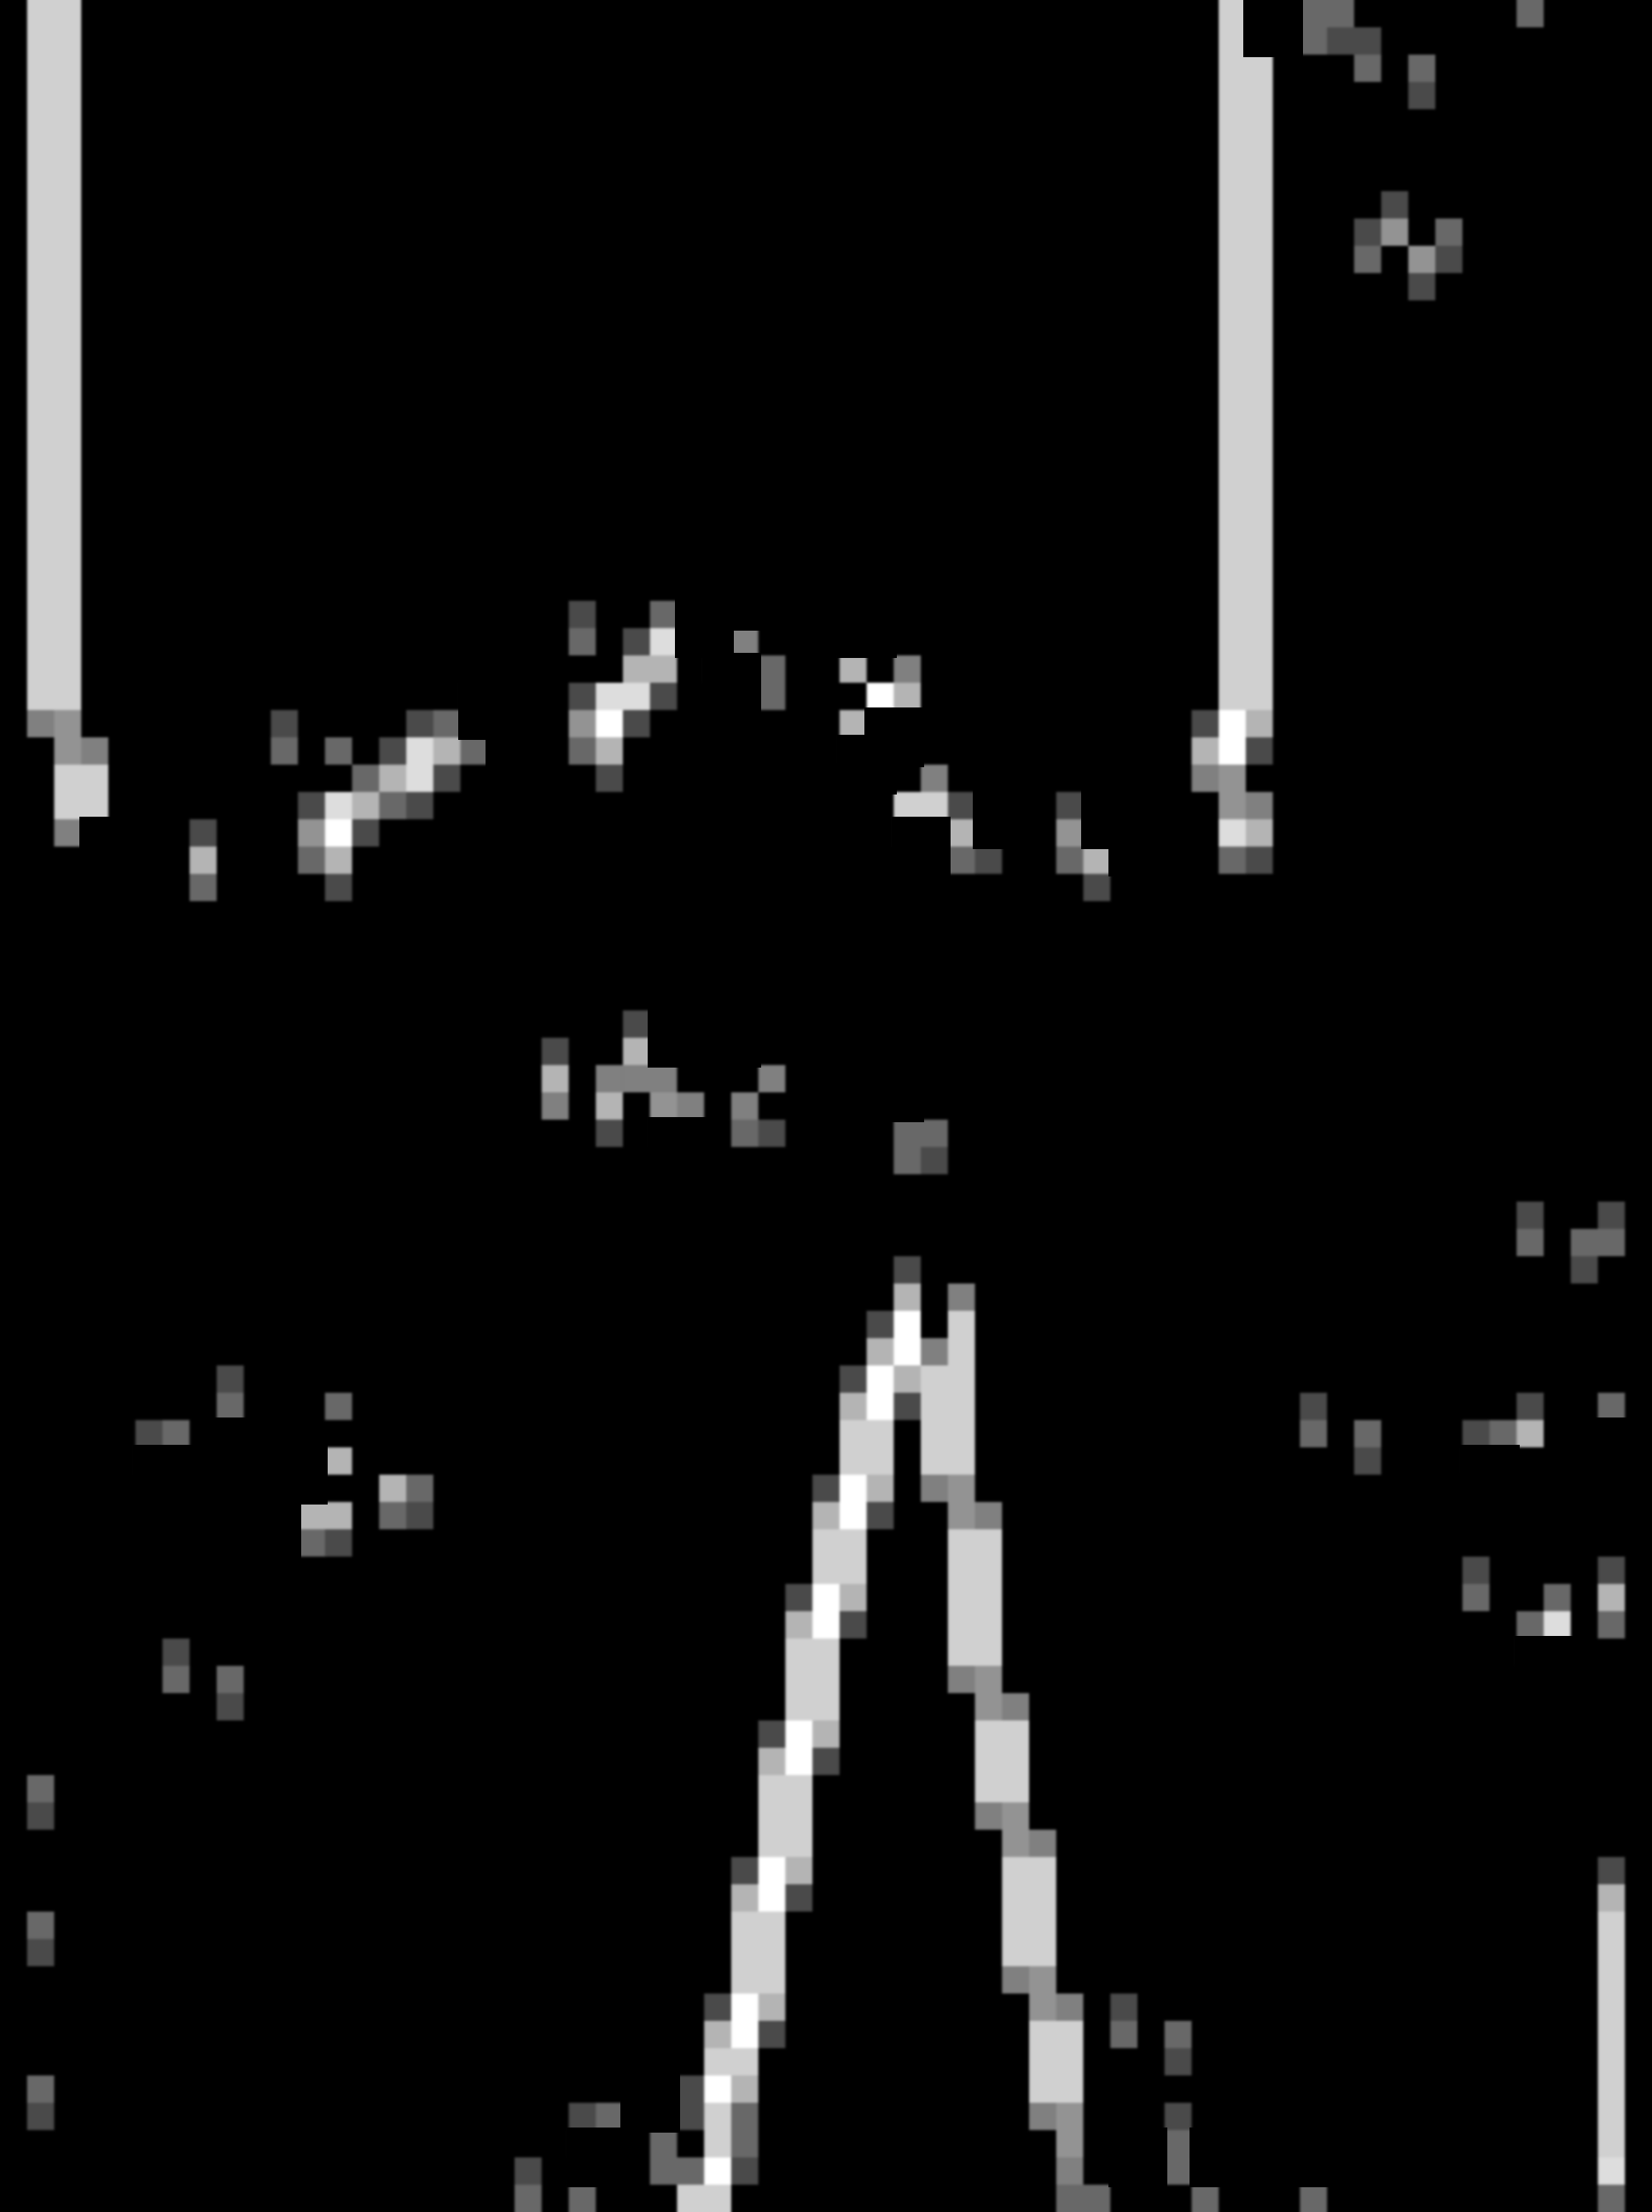
\includegraphics[height=0.5\linewidth]{./fig/sobel_00_00.png}
}
\subfigure[]{
\label{fig:dt}
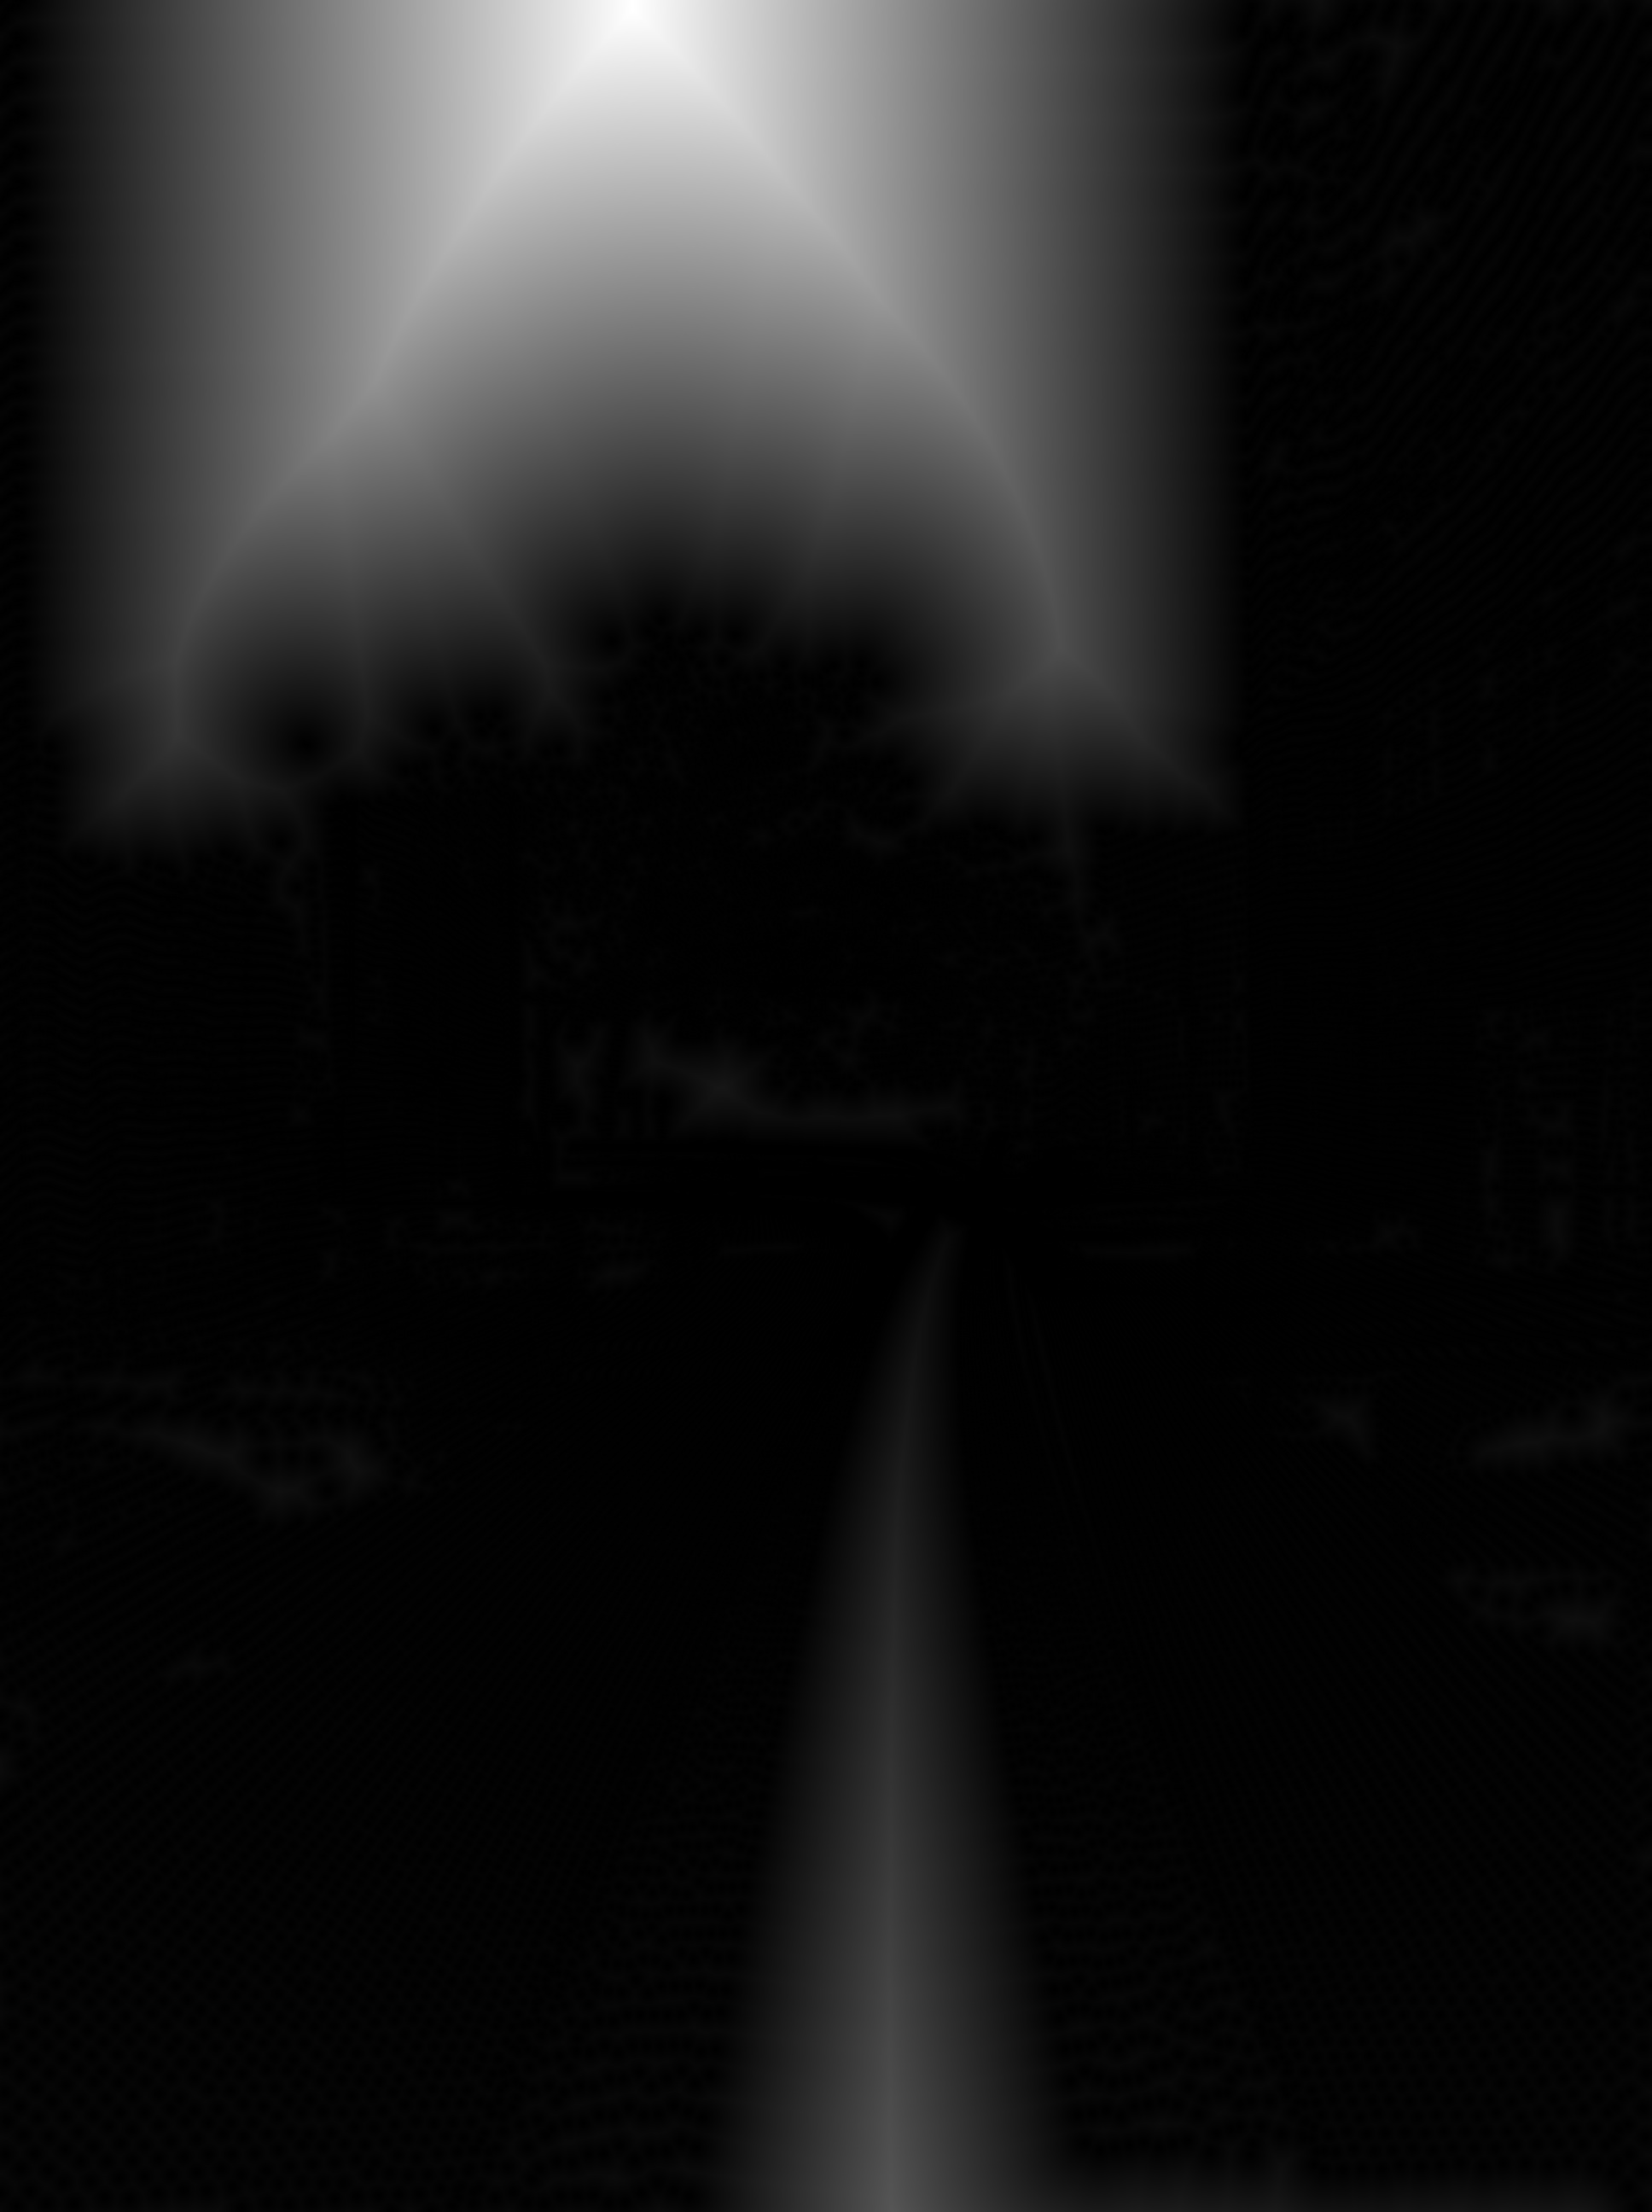
\includegraphics[height=0.5\linewidth]{./fig/dt_00_00.jpg}
}
\end{center}
\caption{The use of the scan points. (a) Boundary of the Scan
  Points. (b) Distance Transform of Scan Point image.}
\label{fig:data_usage}
\end{figure}

\section{Experiment}
\label{sec:exp}

The first experiment is done using GrabCut. As mentioned in previous section, we only use the distance transform image derived from laser point projections as an initialization for MRF in this case. The distance transform image is thresholded to form an initial labeling strategy for foreground and background. As a result, the extra information provided is not used across iterations. The result is shown in Figure~\ref{fig-grab-00_00}. 

\begin{figure}[h]
\begin{center}
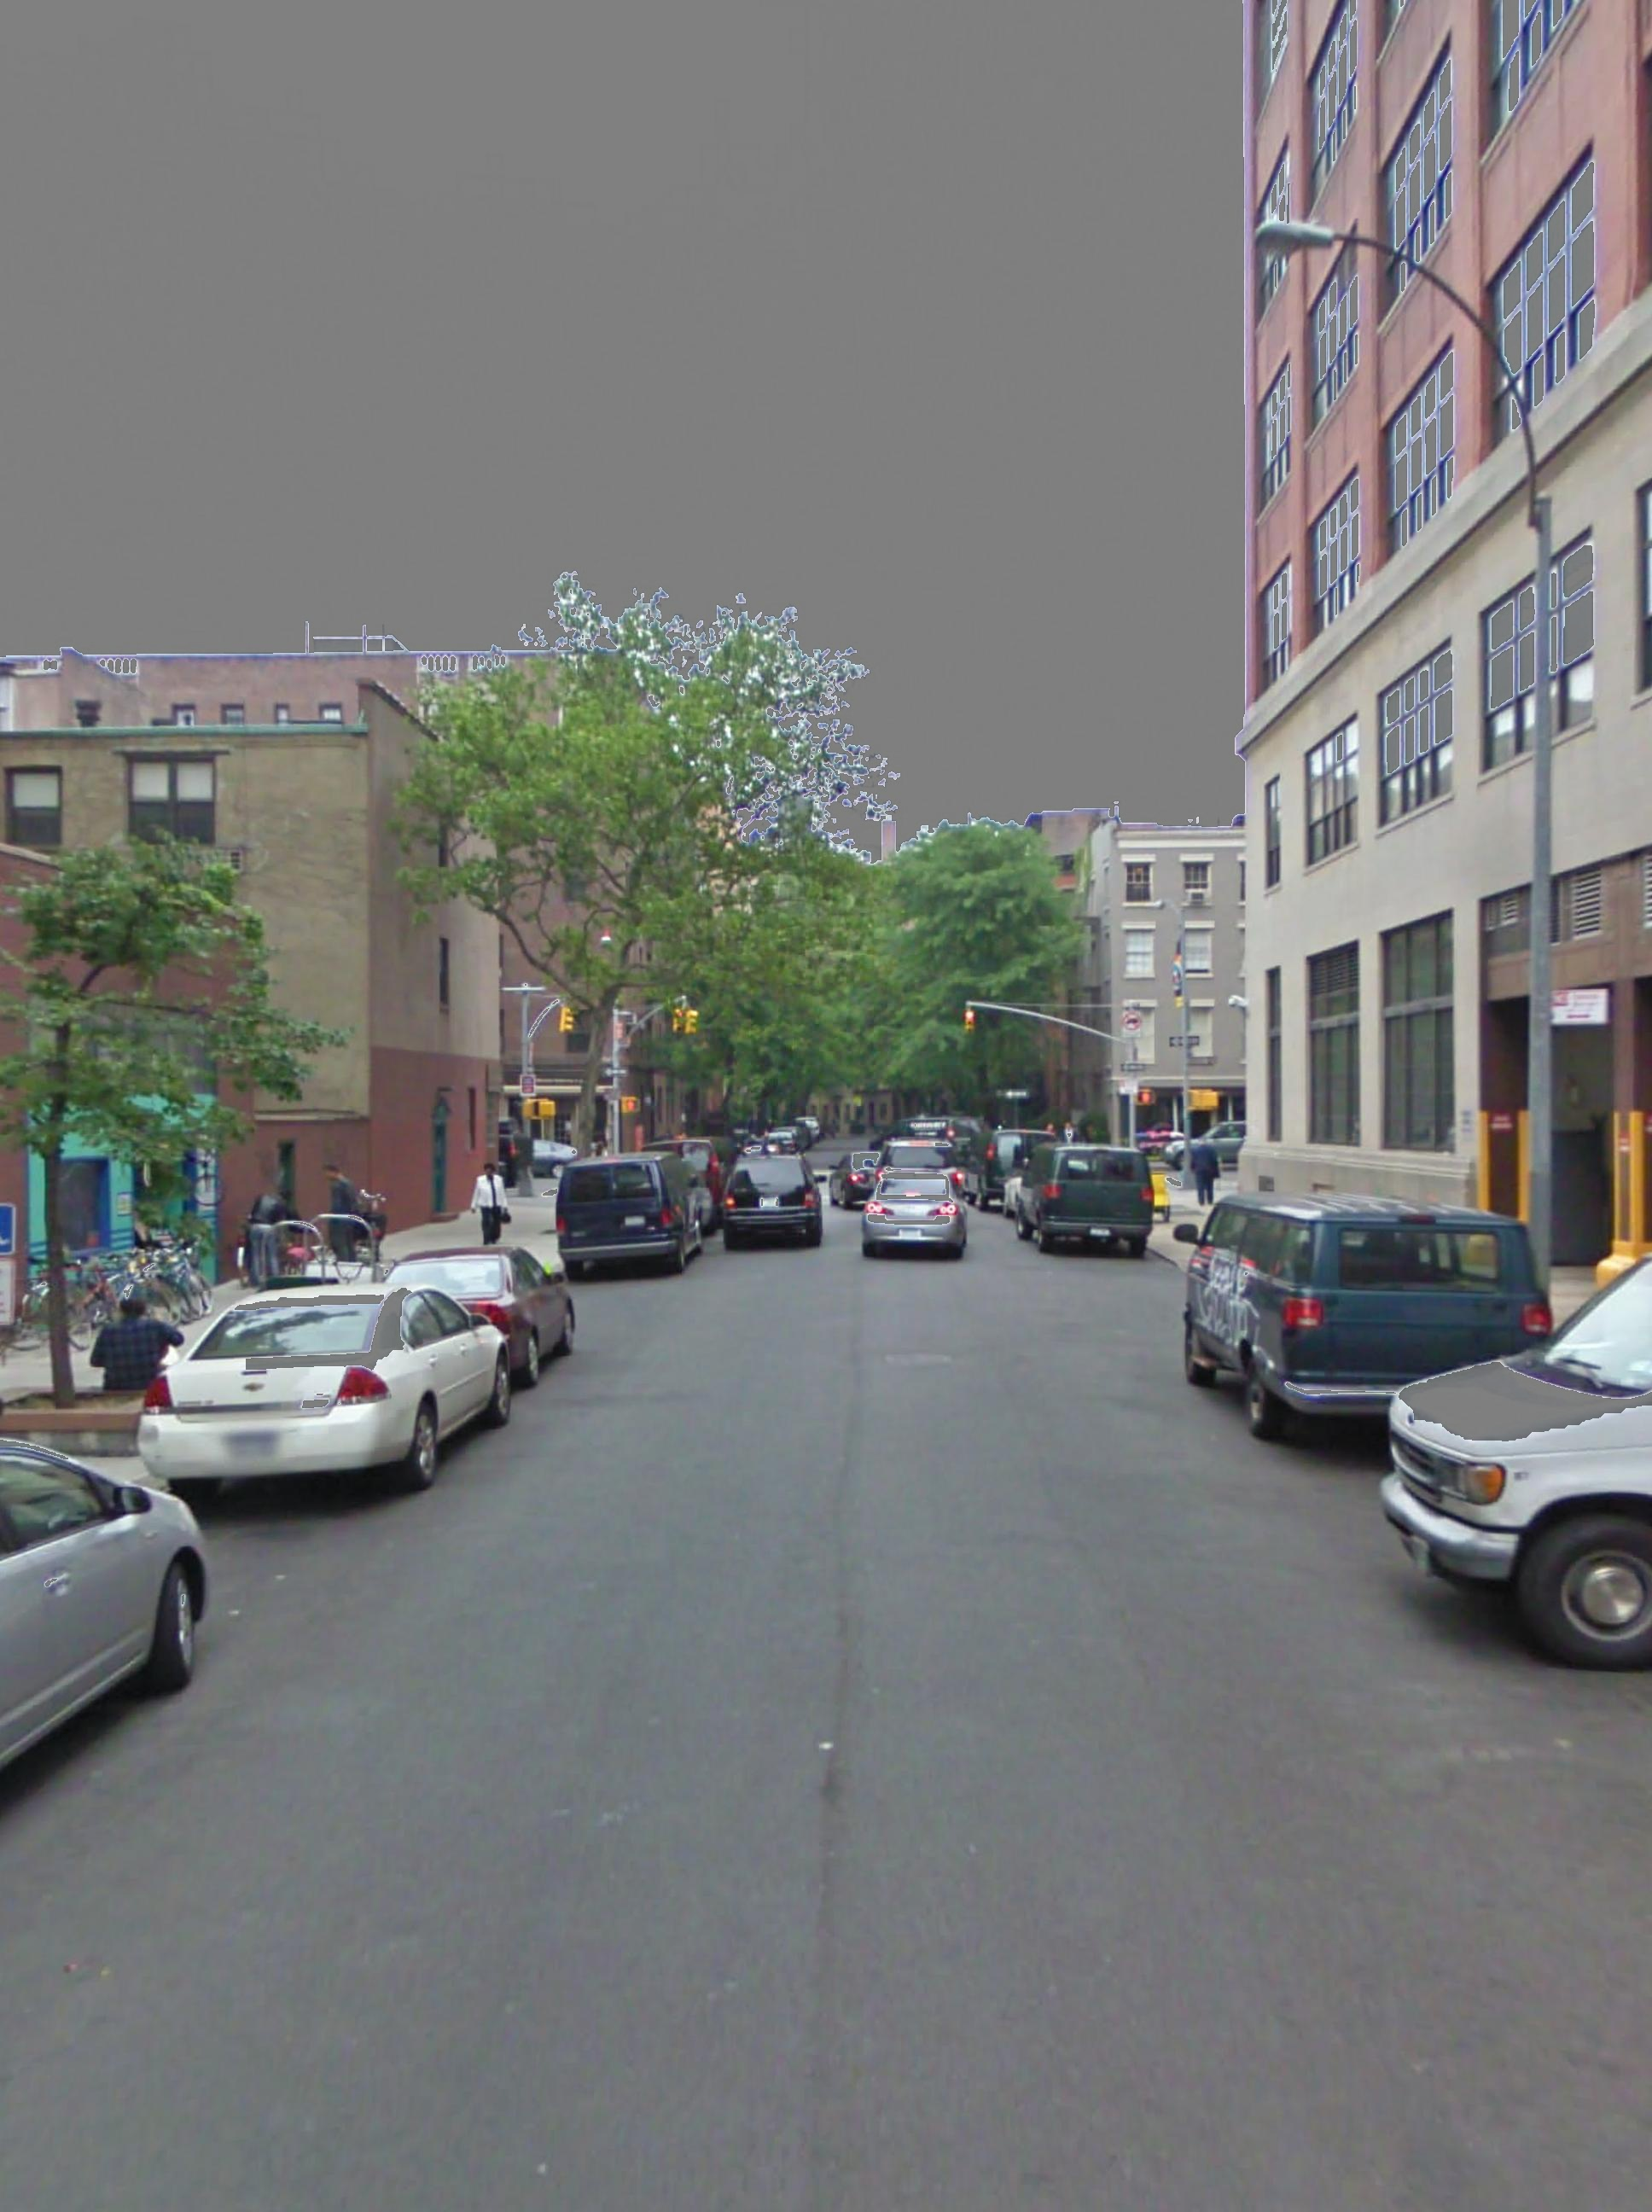
\includegraphics[height=0.5\linewidth]{./fig/overlay_00_00_grab.jpg}
\end{center}
\caption{Segmentation result with GrabCut.}
\label{fig-grab-00_00}
\end{figure}

Note that since we assigned equal cost to edges across the image, cars and windows sharing the similar color as the sky would be segmented as the background.

Having observed this drawback, we decided to vary the cut cost according to our initial estimation of the segments. Note that, assuming foreground objects got scanned more often than background, the natural boundaries would occur at the transition between dense and sparse areas of projected LiDAR points. Thus, in the second experiment, LaserCut, we prepross the distance transform by running simple edge detection algorithm (i.e. Sobel operator) to extract possible boundaries between foreground and background. Therefore, for regions within the potential boundaries, some color differences would be tolerated by assigning smaller weights before the corresponding term in the energy funciton. In contrast, for pixels close to potential boundaries, we intend to rely more on color differences via larger weights to refine the boundary curve. The result is shown in Figure~\ref{fig-laser-00_00}.

\begin{figure}[h]
\begin{center}
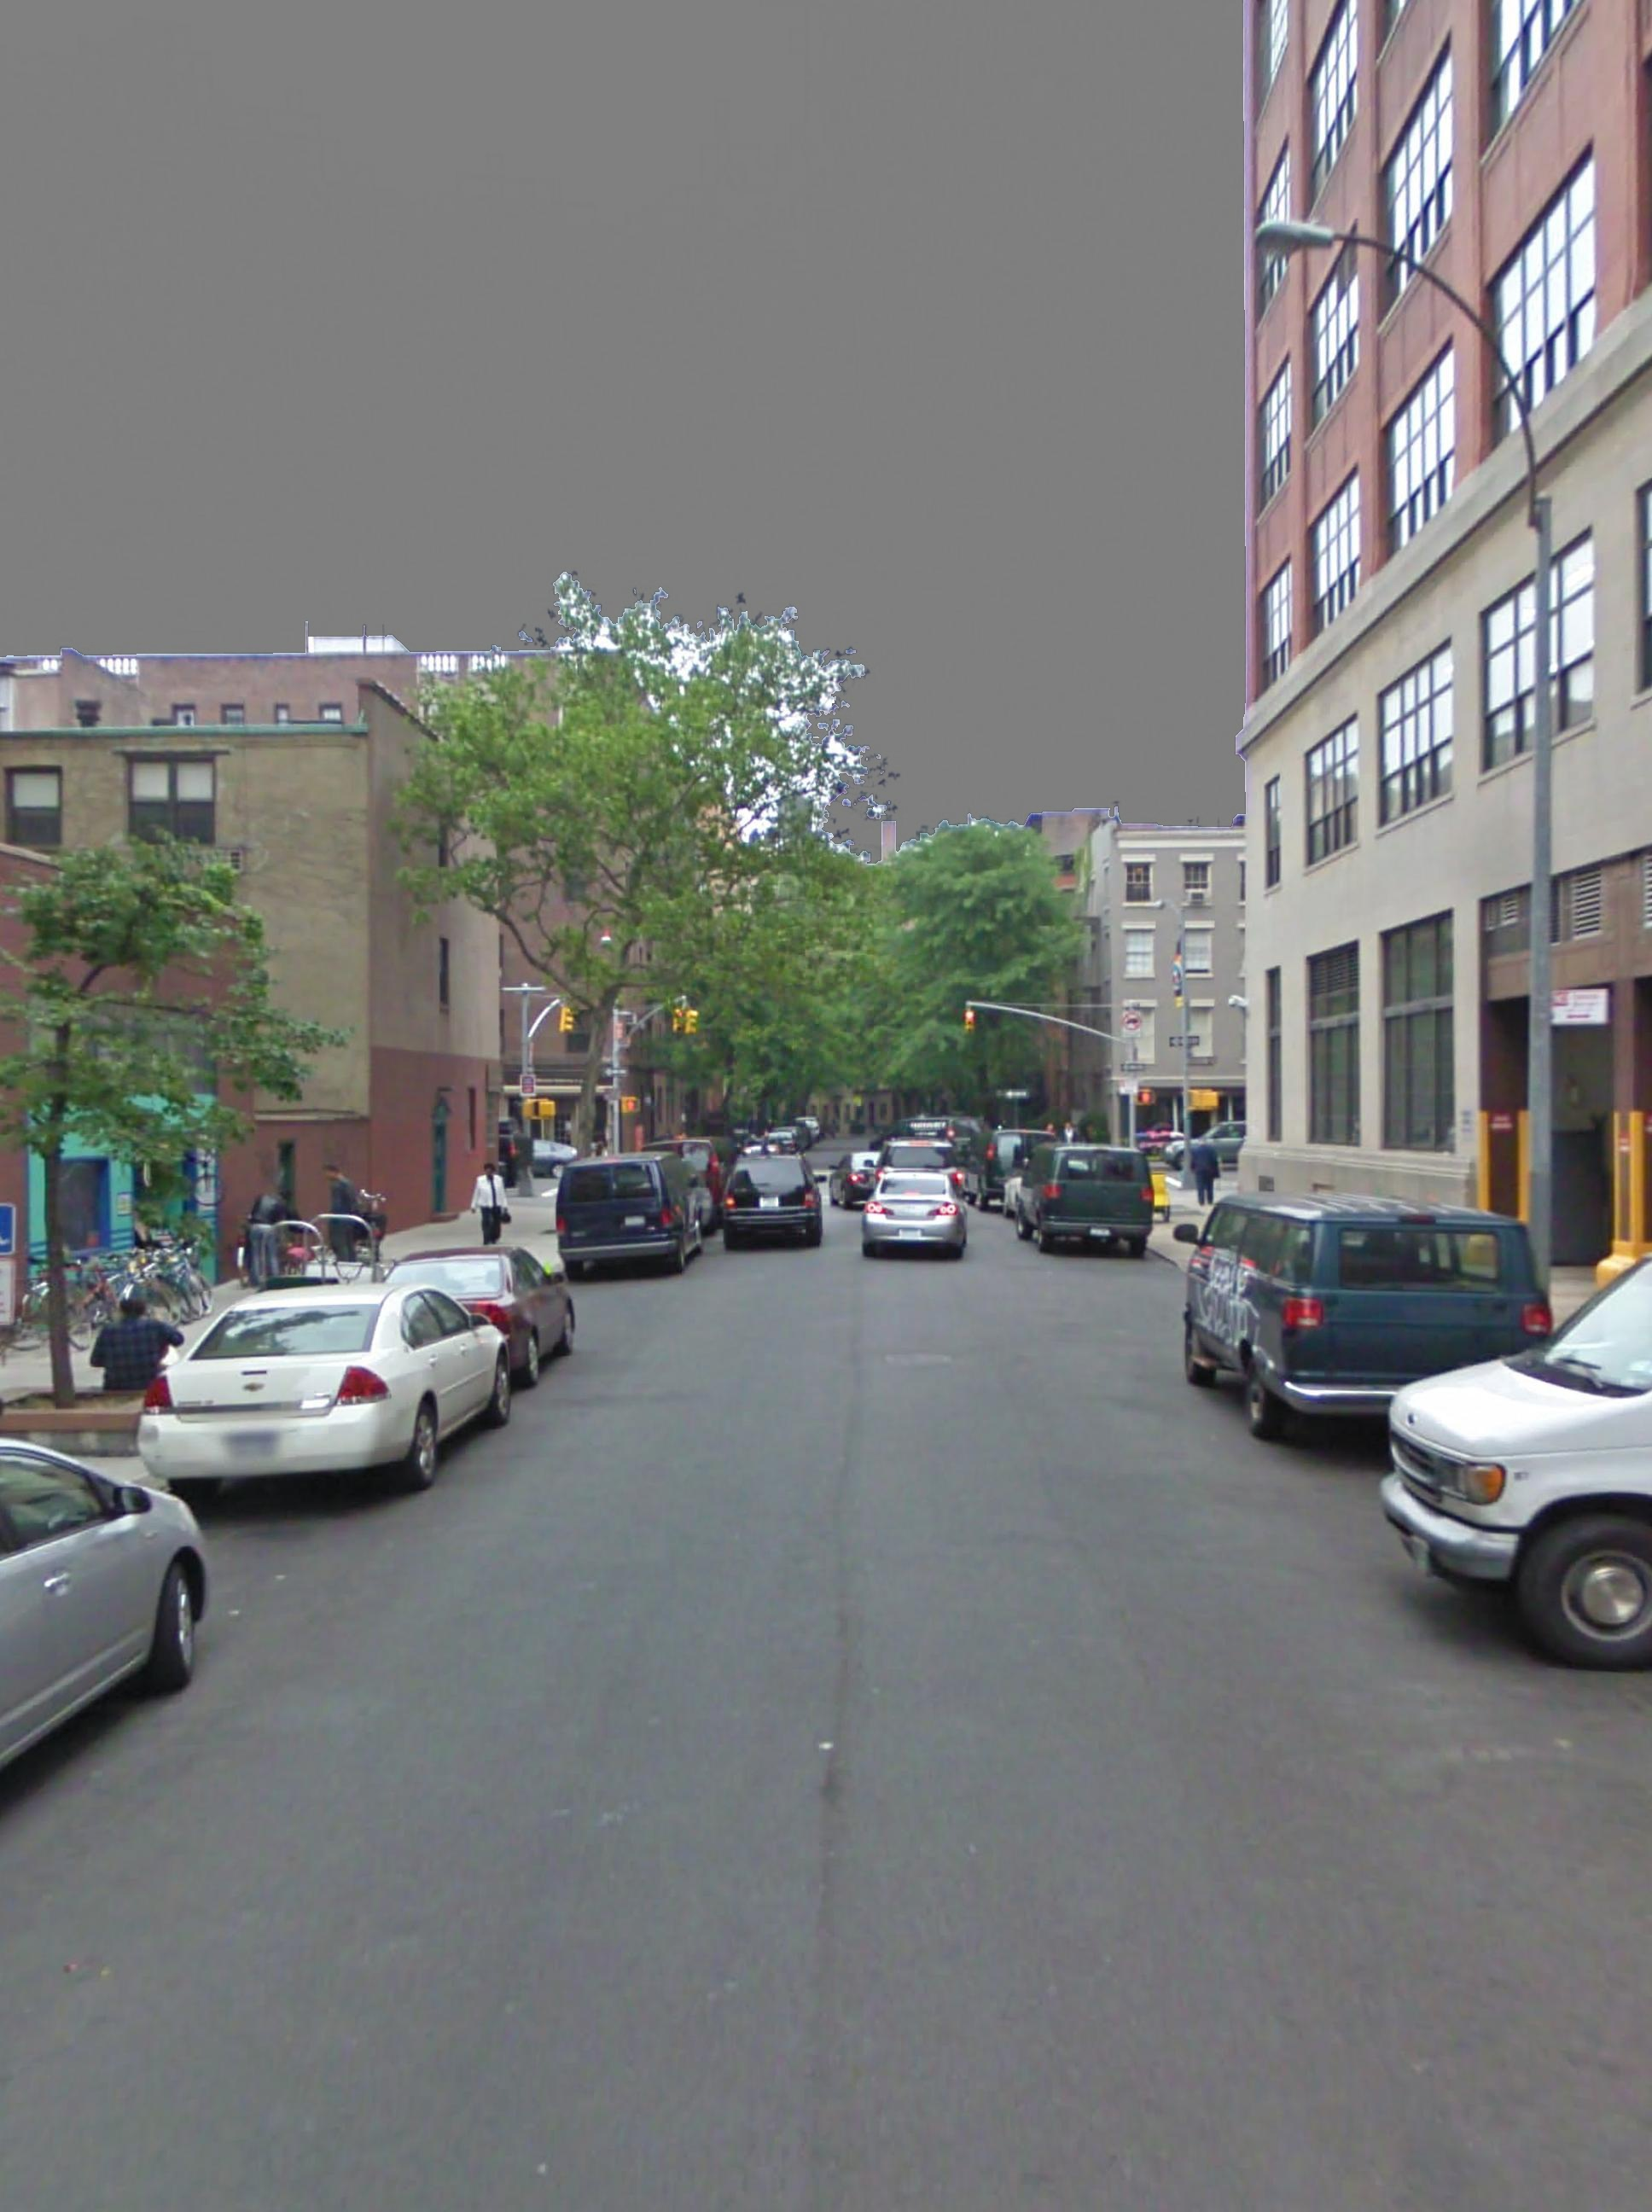
\includegraphics[height=0.5\linewidth]{./fig/overlay_00_00_laser.jpg}
\end{center}
\caption{Segmentation result with LaserCut.}
\label{fig-laser-00_00}
\end{figure}

Comparing to GrabCut model, we successfully eliminated the white cars in the front from the background.

To further evaluate our model, we did another experiment on the same image with a widely used MRF model, Ising model. In this setting, color difference between neighboring pixels is completely ignored by assigning the same cost for connectivity to all edges in the MRF graph. The result is shown in Figure~\ref{fig-ising-00_00}.

\begin{figure}[h]
\begin{center}
\subfigure[Large threshold on initialization]{
\label{fig-ising-large}
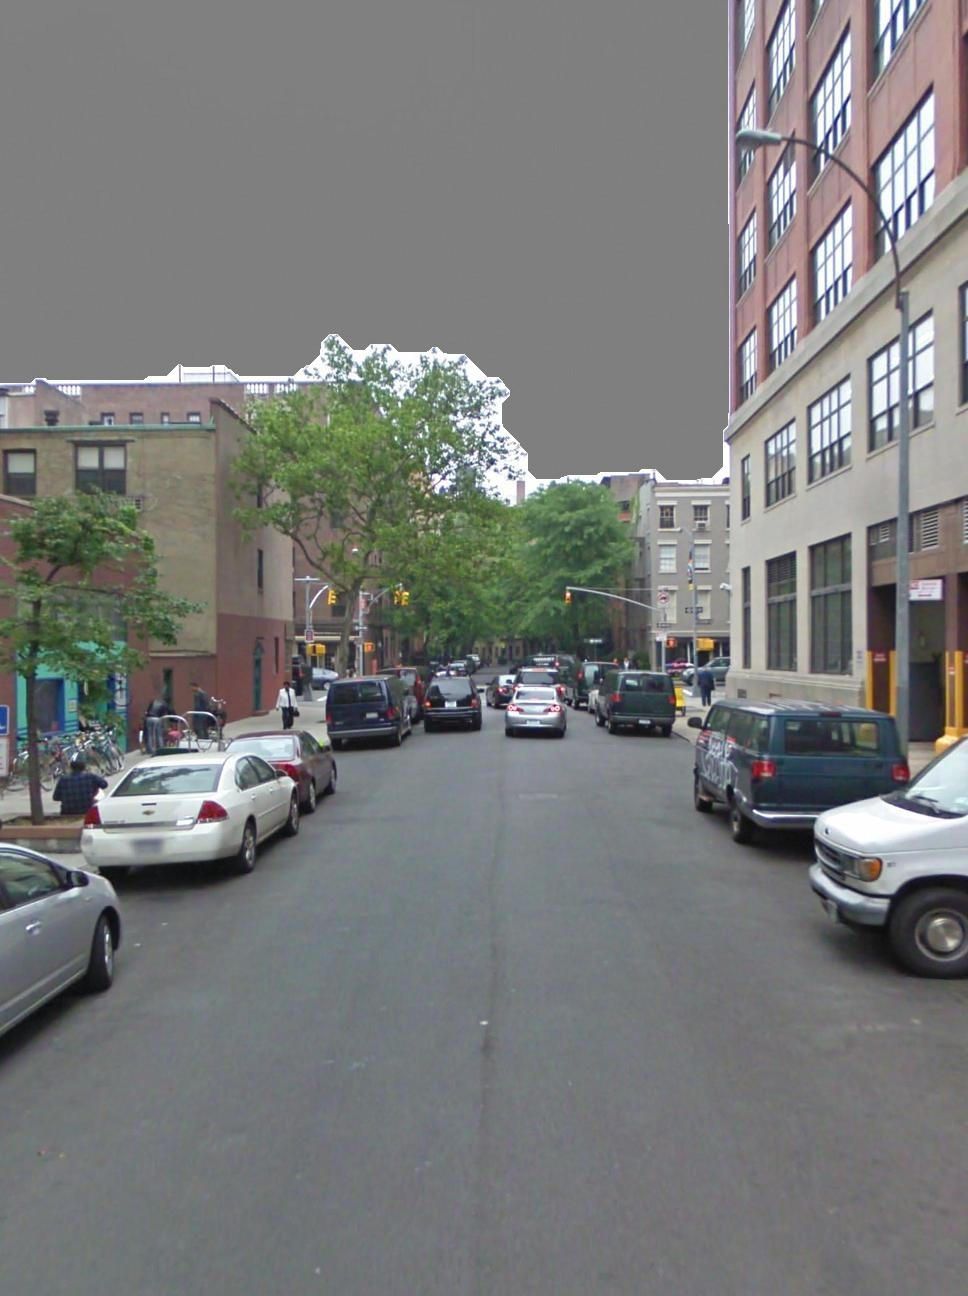
\includegraphics[height=0.5\linewidth]{./fig/overlay_00_00_ising_large.jpg}
}
\subfigure[Small threshold on initialization]{
\label{fig-ising-small}
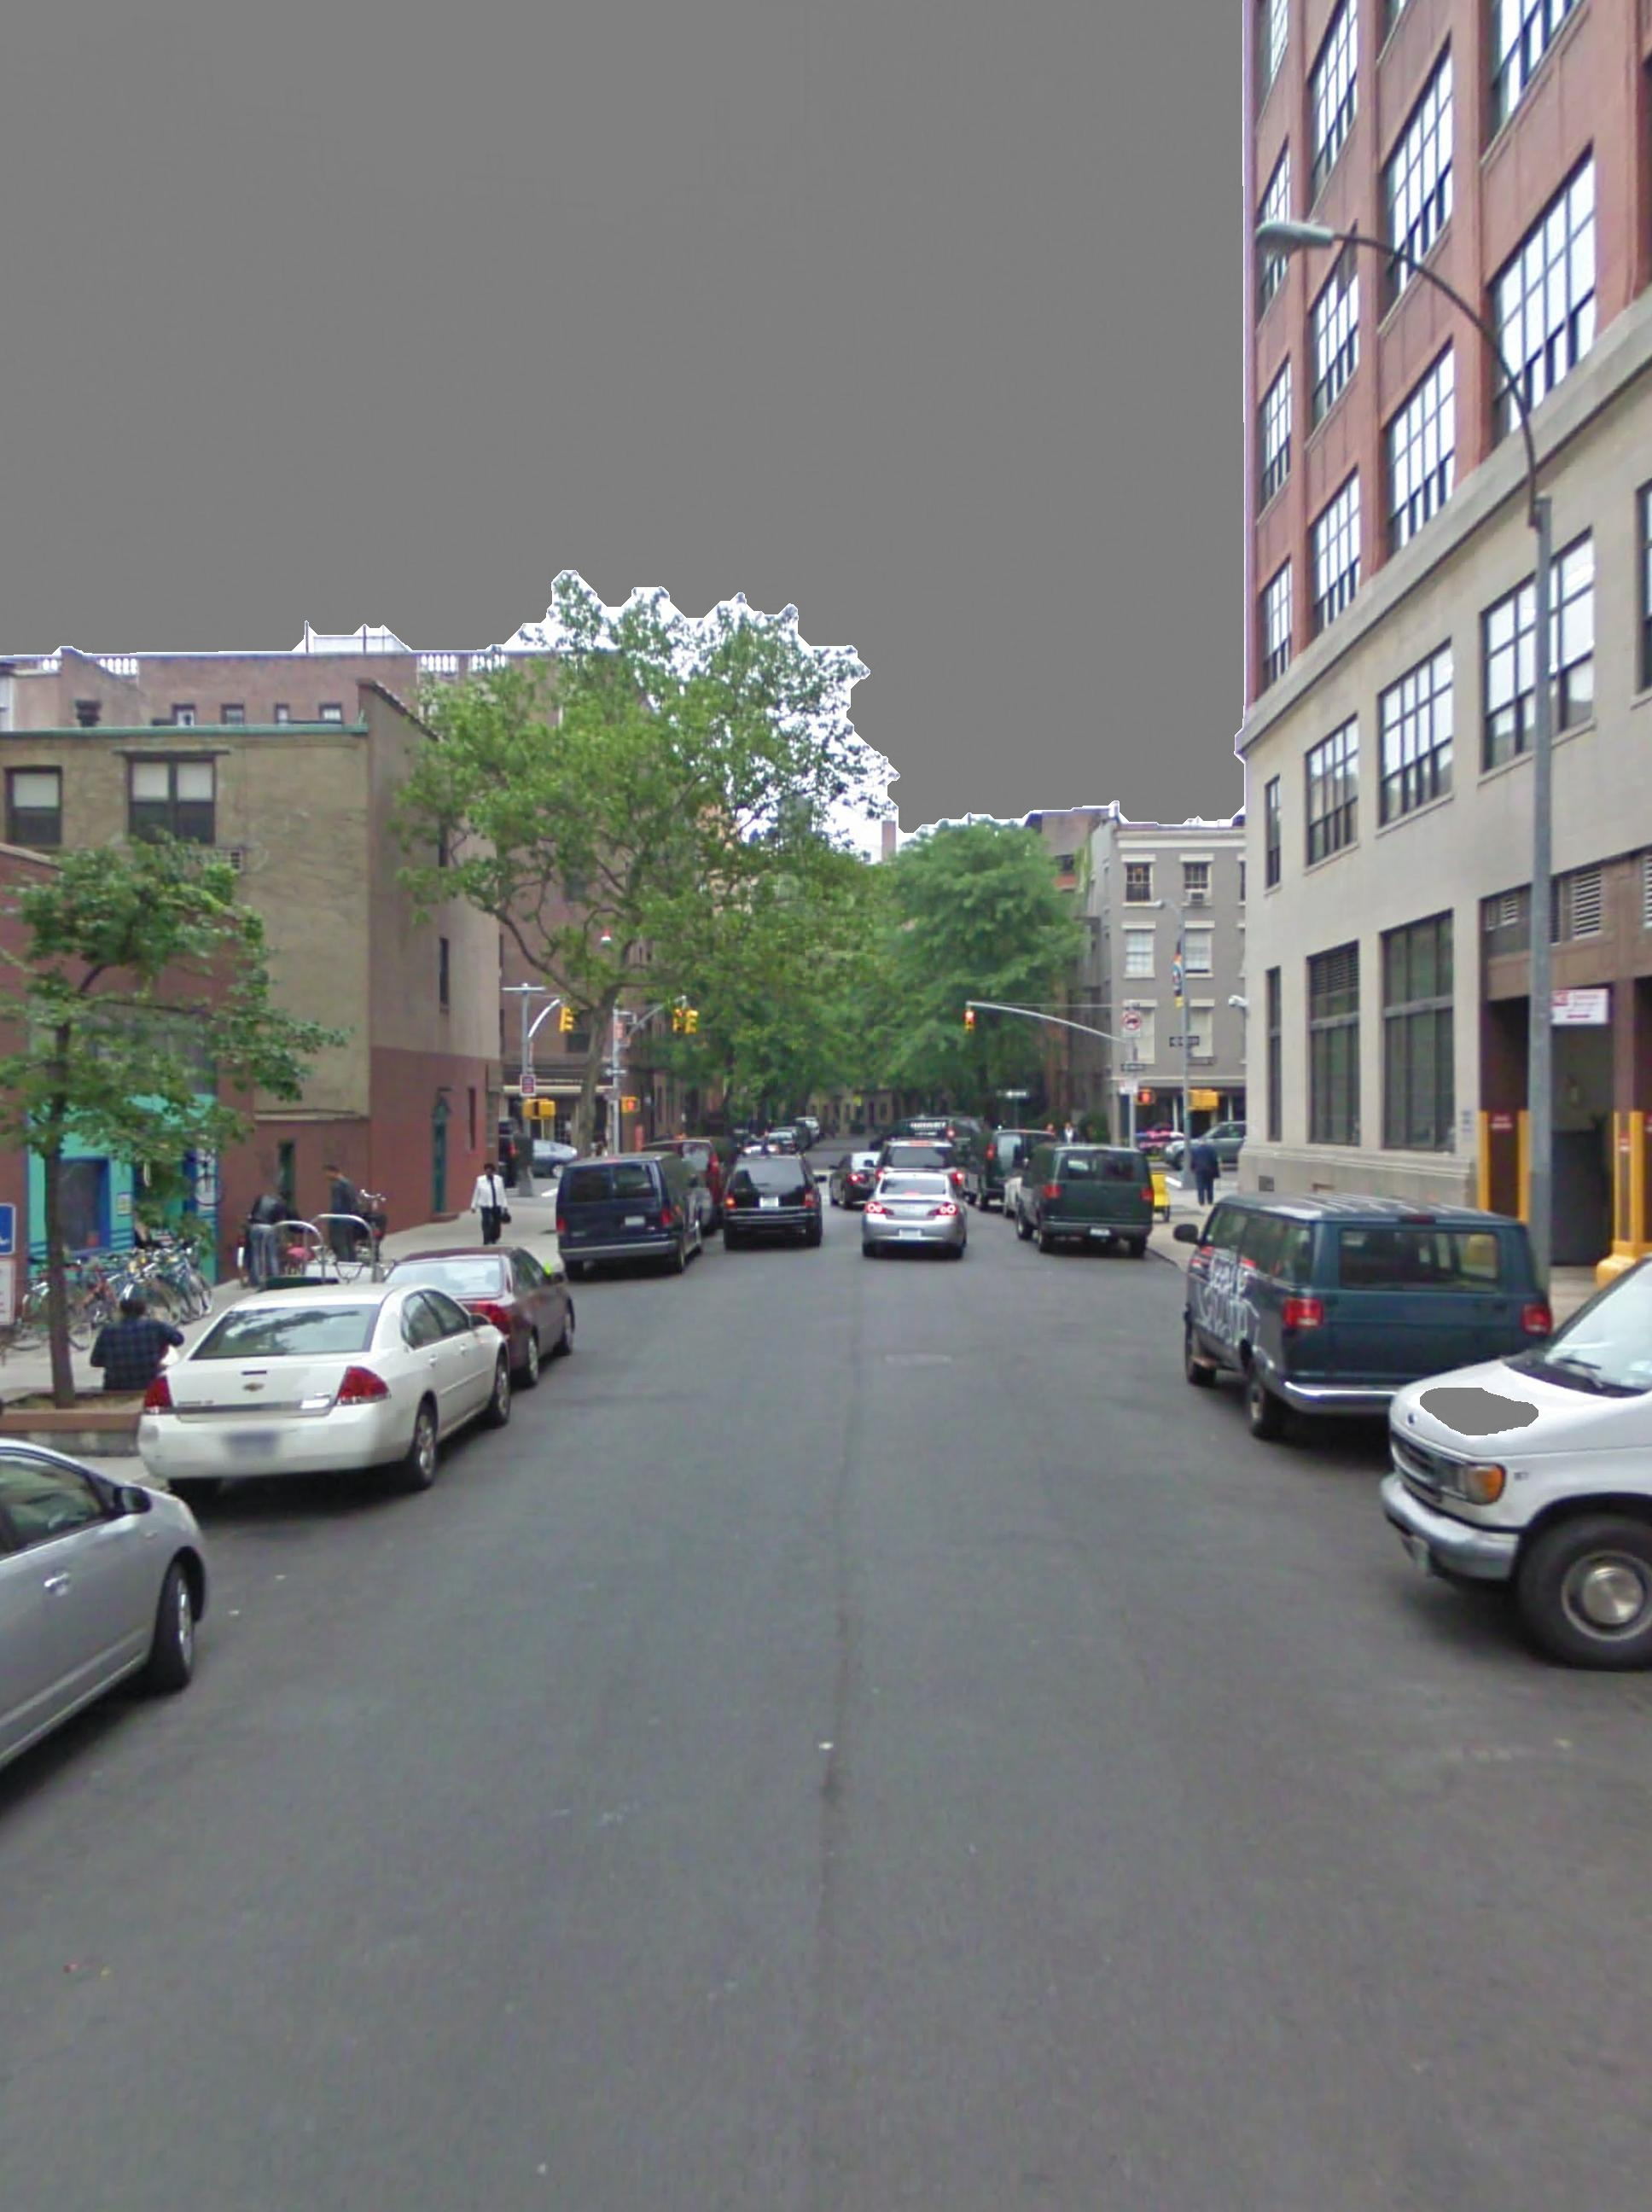
\includegraphics[height=0.5\linewidth]{./fig/overlay_00_00_ising_small.jpg}
}
\end{center}
\caption{Segmentation result with Ising Model.}
\label{fig-ising-00_00}
\end{figure}

Taking a close look at the boundary Ising model found, we observed that the foreground objects are outlined by a ``margin" of the sky. This is probably due to we only used Gaussian mixture model to measure the clustering in color. Since there are white cars on the road, the GMM would intend to label part of the sky as the foreground due to larger threshold~\ref{fig-ising-large} on distance transform image. However, smaller threshold~\ref{fig-ising-small} values would result in labeling the white cars in the front to background initial, which would be generally hard to correct in later iteration under this model.

\section{Evaluation}

In general, evaluating segmentation result is hard due to the absence of precise quantitative measurement without ground truth. In addition, there is another important issue centers around the use of energy to compare energy minimization algorithms. The goal in computer vision is not to compute the lowest energy but the most accurate one, besides computing the global minimum was shown to be NP-complete in general~\citep{Boykov2001Fast}. In the paper by~\citet{Szeliski2008Comparative}, a quantitative comparison between lowest energy achieved by different energy minimization algorithms and the energy calculated from ground truth provides experimental proof for this argument. Although one can argue that we could manually draw the boundaries for each image we used in this project, due to high resolution (1936 x 2592) and limited size of sample labling from different users we can account for given the time, the accuracy and unbiasness of the ground truth cannot be guaranteed.

As an alternative, we decided to conduct a comparison study among the three experiments we did mentioned in previous section. The best model we have is LaserCut which has the advantage of adaptiveness of initial guess through out all iterations. As we discussed before, comparing to GrabCut model, LaserCut successfully classified the cars with similar color as the background as part of the foreground. This observation suggests the effectiveness of adaptively using extra information acquired from LiDAR scan. On the other hand, comparing to Ising model, LaserCut could provide more complicated and accurate boundary between foreground and background, which indicates the effectiveness of separation on color differences when close to the boundary.

Granted, there are still areas near the boundary being mislabelled, for instance, some leaves of the tree in Figure~\ref{fig-laser-00_00}. It is generally hard to determine the exact bounday of such complicated foreground object. Even when we have captured images with such high resolution, it is still far from certain that all the details of objects far back to the scene can be accurately preserved. Moreover, even though we can somehow manage to obtain all the details in the scene, the correctness of boundaries around complicated objects like trees would be rather subjective to different people.

Therefore, in spite of the fact that most of the model evaluation is based on visual check in this project, we hope our observations and analysis could make a plausible case for the advantage of LaserCut model over the others.

\section{Lesson Learnt}
 Through careful study on the resulting segmentation of our approach,
 we learnt several things about the algorithm.
 For one thing, color feature helps to produce a good approximation to the
 \emph{true} boundary between foreground and background. 
 In Figure~\ref{fig-laser-00_00}, the curve of ``background'' is very close to
 the truth boundary between green leaves and sky. From the distance
 data, we can see there are not many ``leaves'' pixels with
 distance, therefore we conjecture that the color feature plays an
 important role in delimiting the boundary.
 For the other thing, the algorithm achieves balance between the
 influence of distance data, which is used to generate inital states,
 and the influence of color features, which is used to refine the
 segmentation. 
 For example, in Figure~\ref{fig-laser-00_00}, although the white cars have similar color
 to that of sky, they are not considered as background.  
 Another example is that some sky pixels in the image are classified
 as background, depite the dataset suggests that they have finite
 distance to the camera.  
 These two examples show that we are able to use color feature to fix
 minor errors in the distance data while still maintaining most of
 status generated by the distance data.

\section {Future Work}
Our future work will focus on the following two aspects.
First, the background pixels in our experiment images have very
similar color. This fact greatly helps segmentation as we can put much
weight on the color feature to infer the labels of pixels. In the
future, we want to incoporate images with more colorful
background. To do segmentation on such images, we may have to
introduce new factors to model background and foreground.
The other aspect is to do the general image segmentation. That is,
segment the image into multi-layer. At present, we only use whether
the pixel has a finite distance number or not. As we take the actual
distance value into account, we can segement the images into several
layers, with pixels in the same layers have close distance value.

\section{More Results}
We also did a comparison study on other images to further evaluate our algorithm. 

\begin{figure}[h]
\begin{center}
\subfigure[Original image]{
\label{fig-im_02_02}
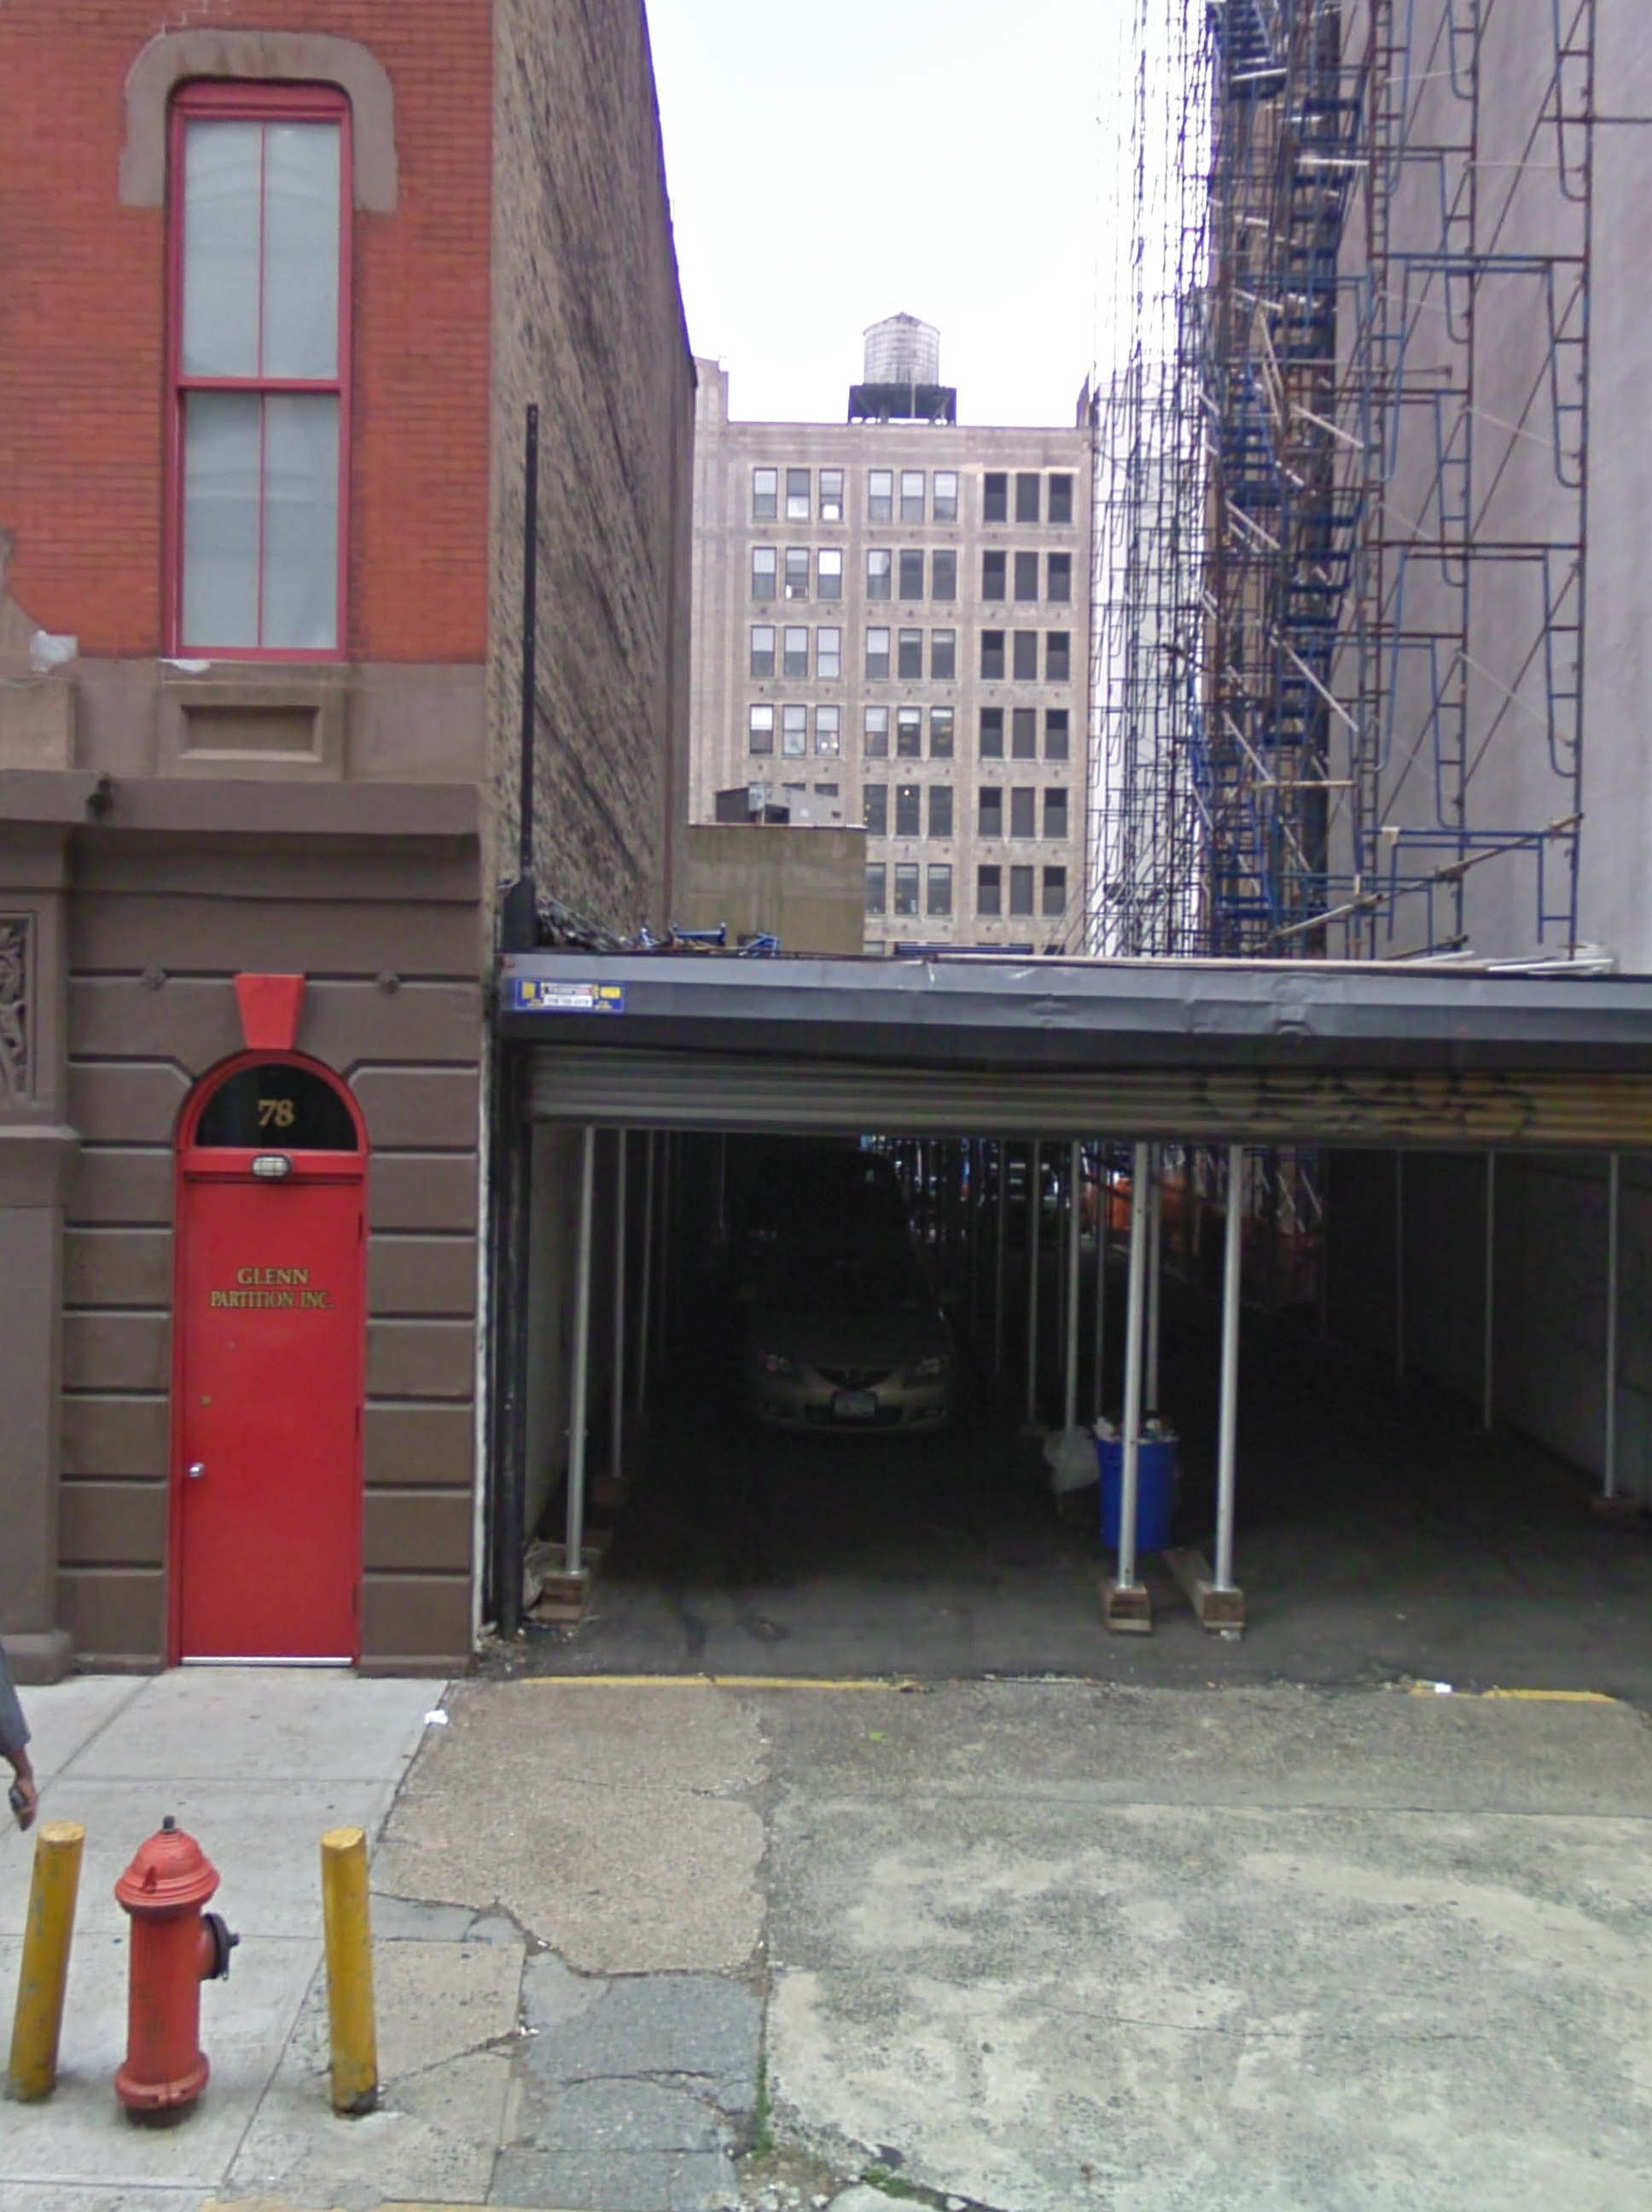
\includegraphics[height=0.3\linewidth]{./fig/image_02_02.jpg}
}
\subfigure[GrabCut]{
\label{fig-gc_02_02}
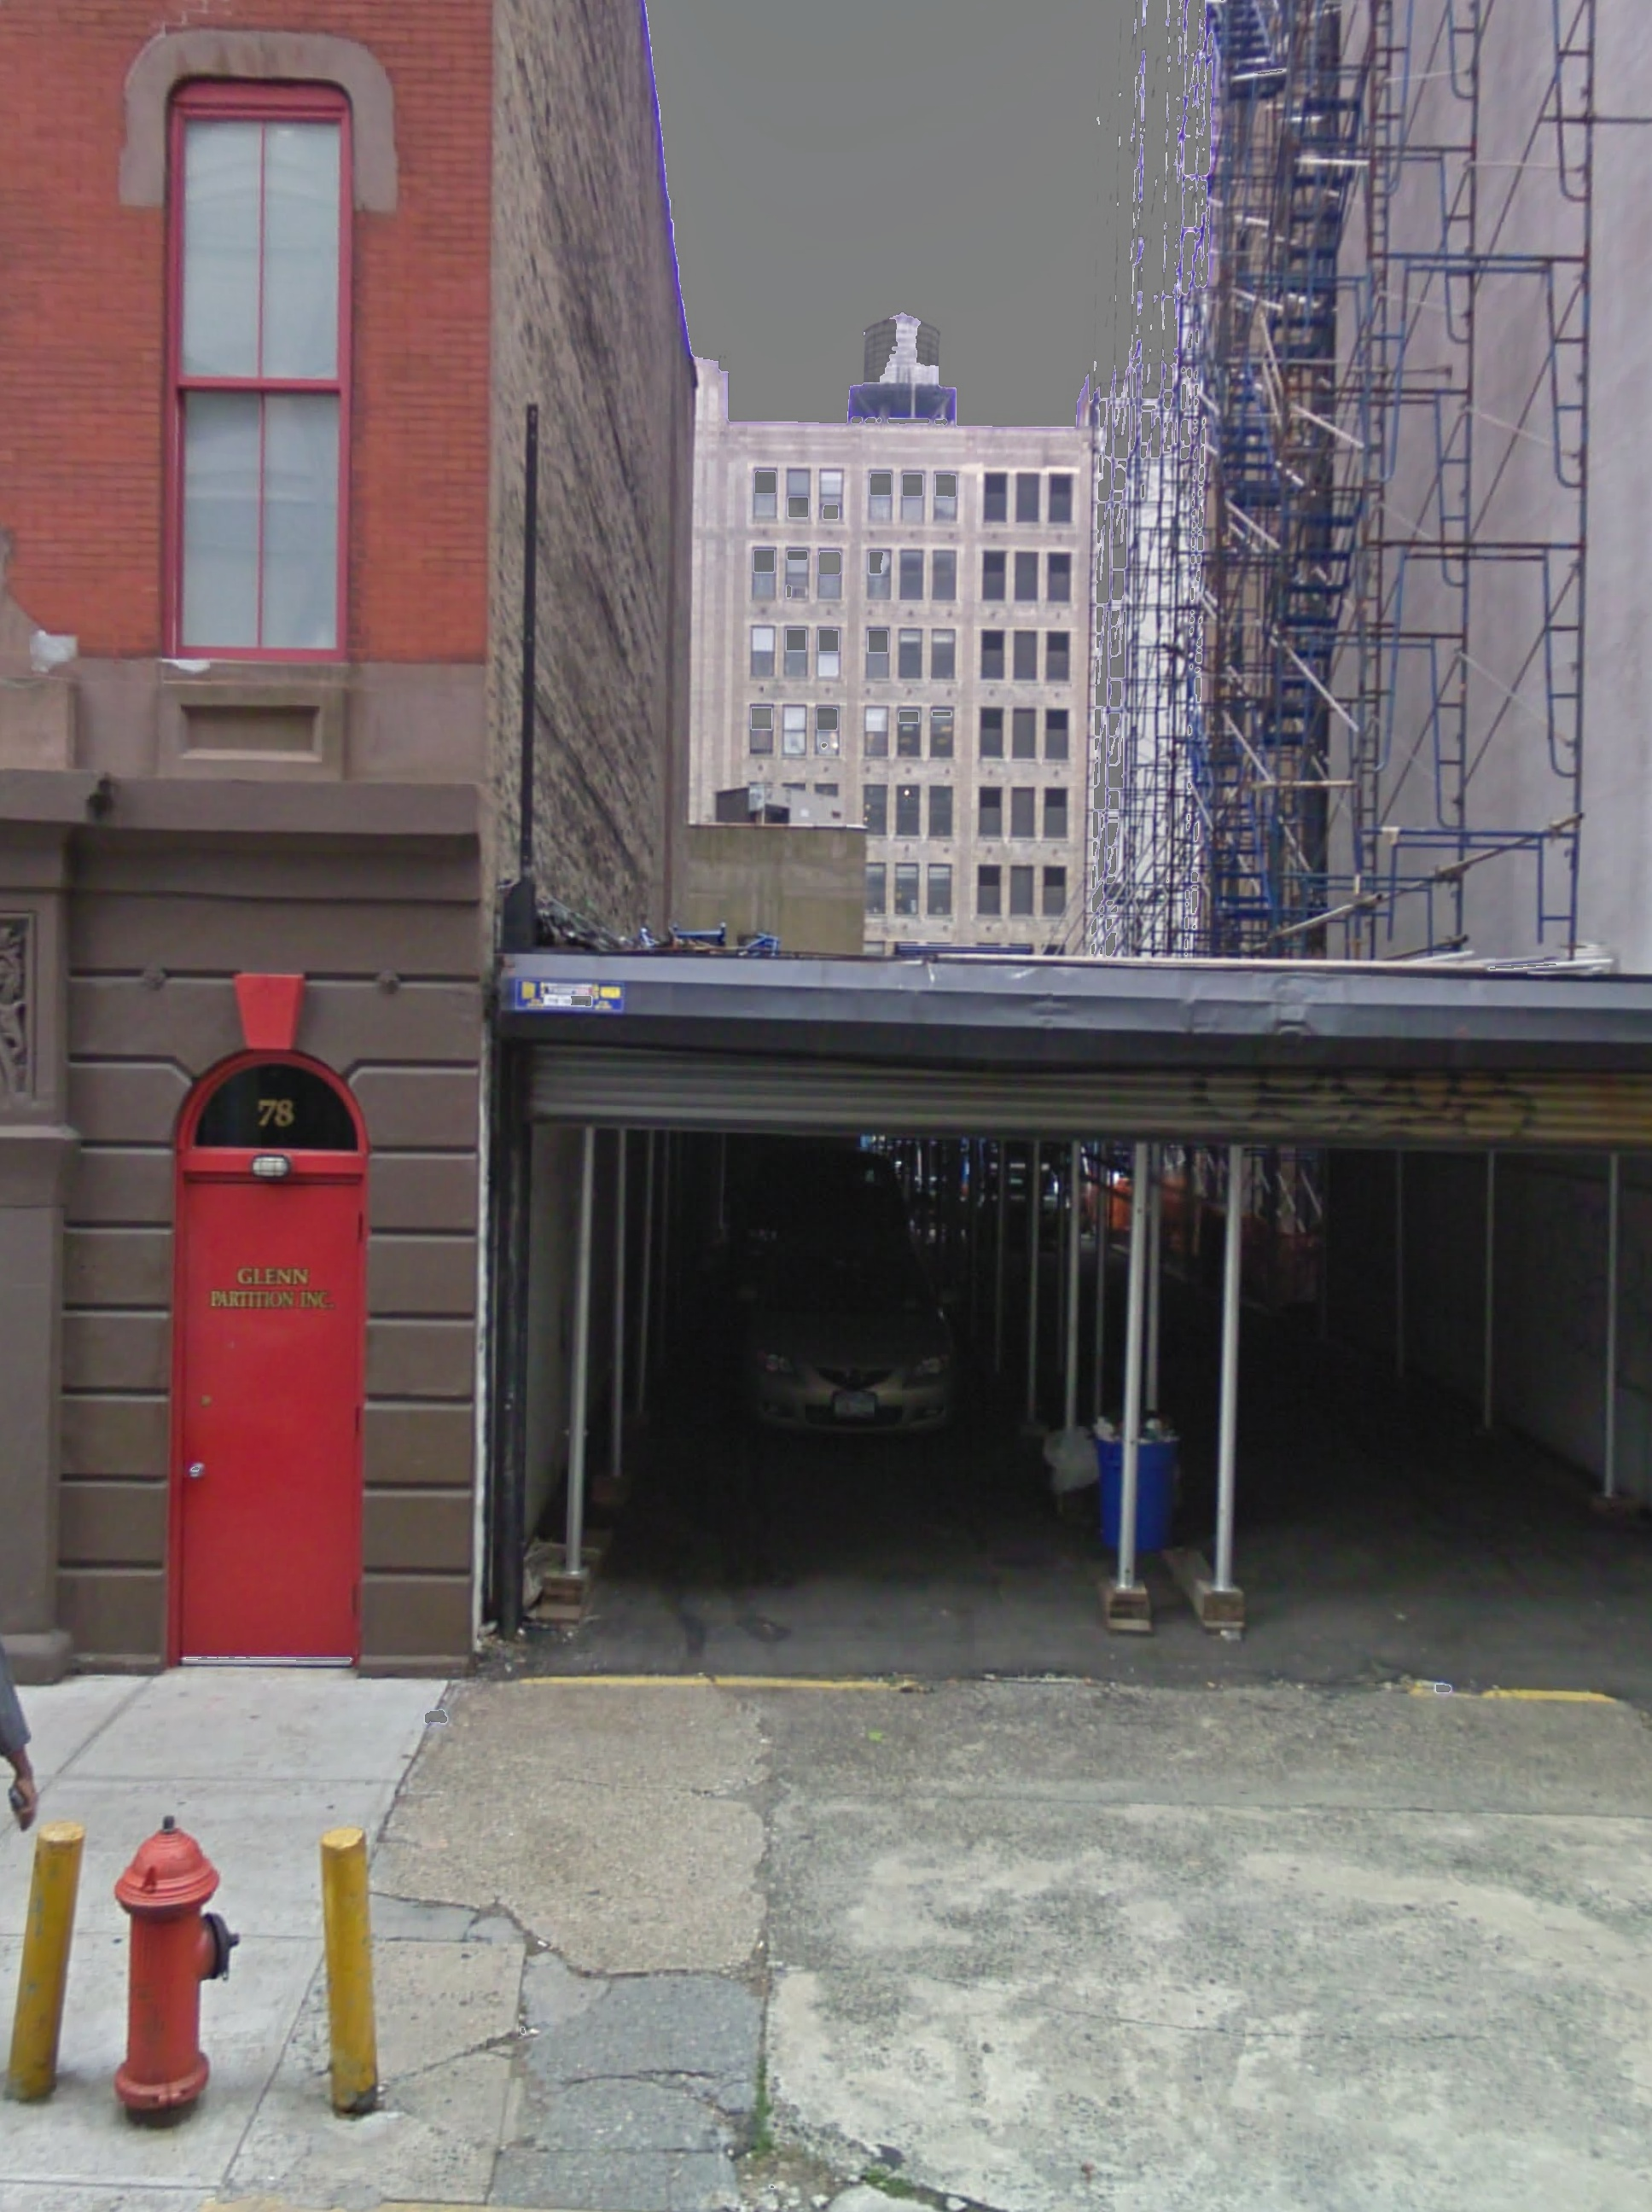
\includegraphics[height=0.3\linewidth]{./fig/overlay_02_02_grab.jpg}
}
\subfigure[Ising Model]{
\label{fig-is_02_02}
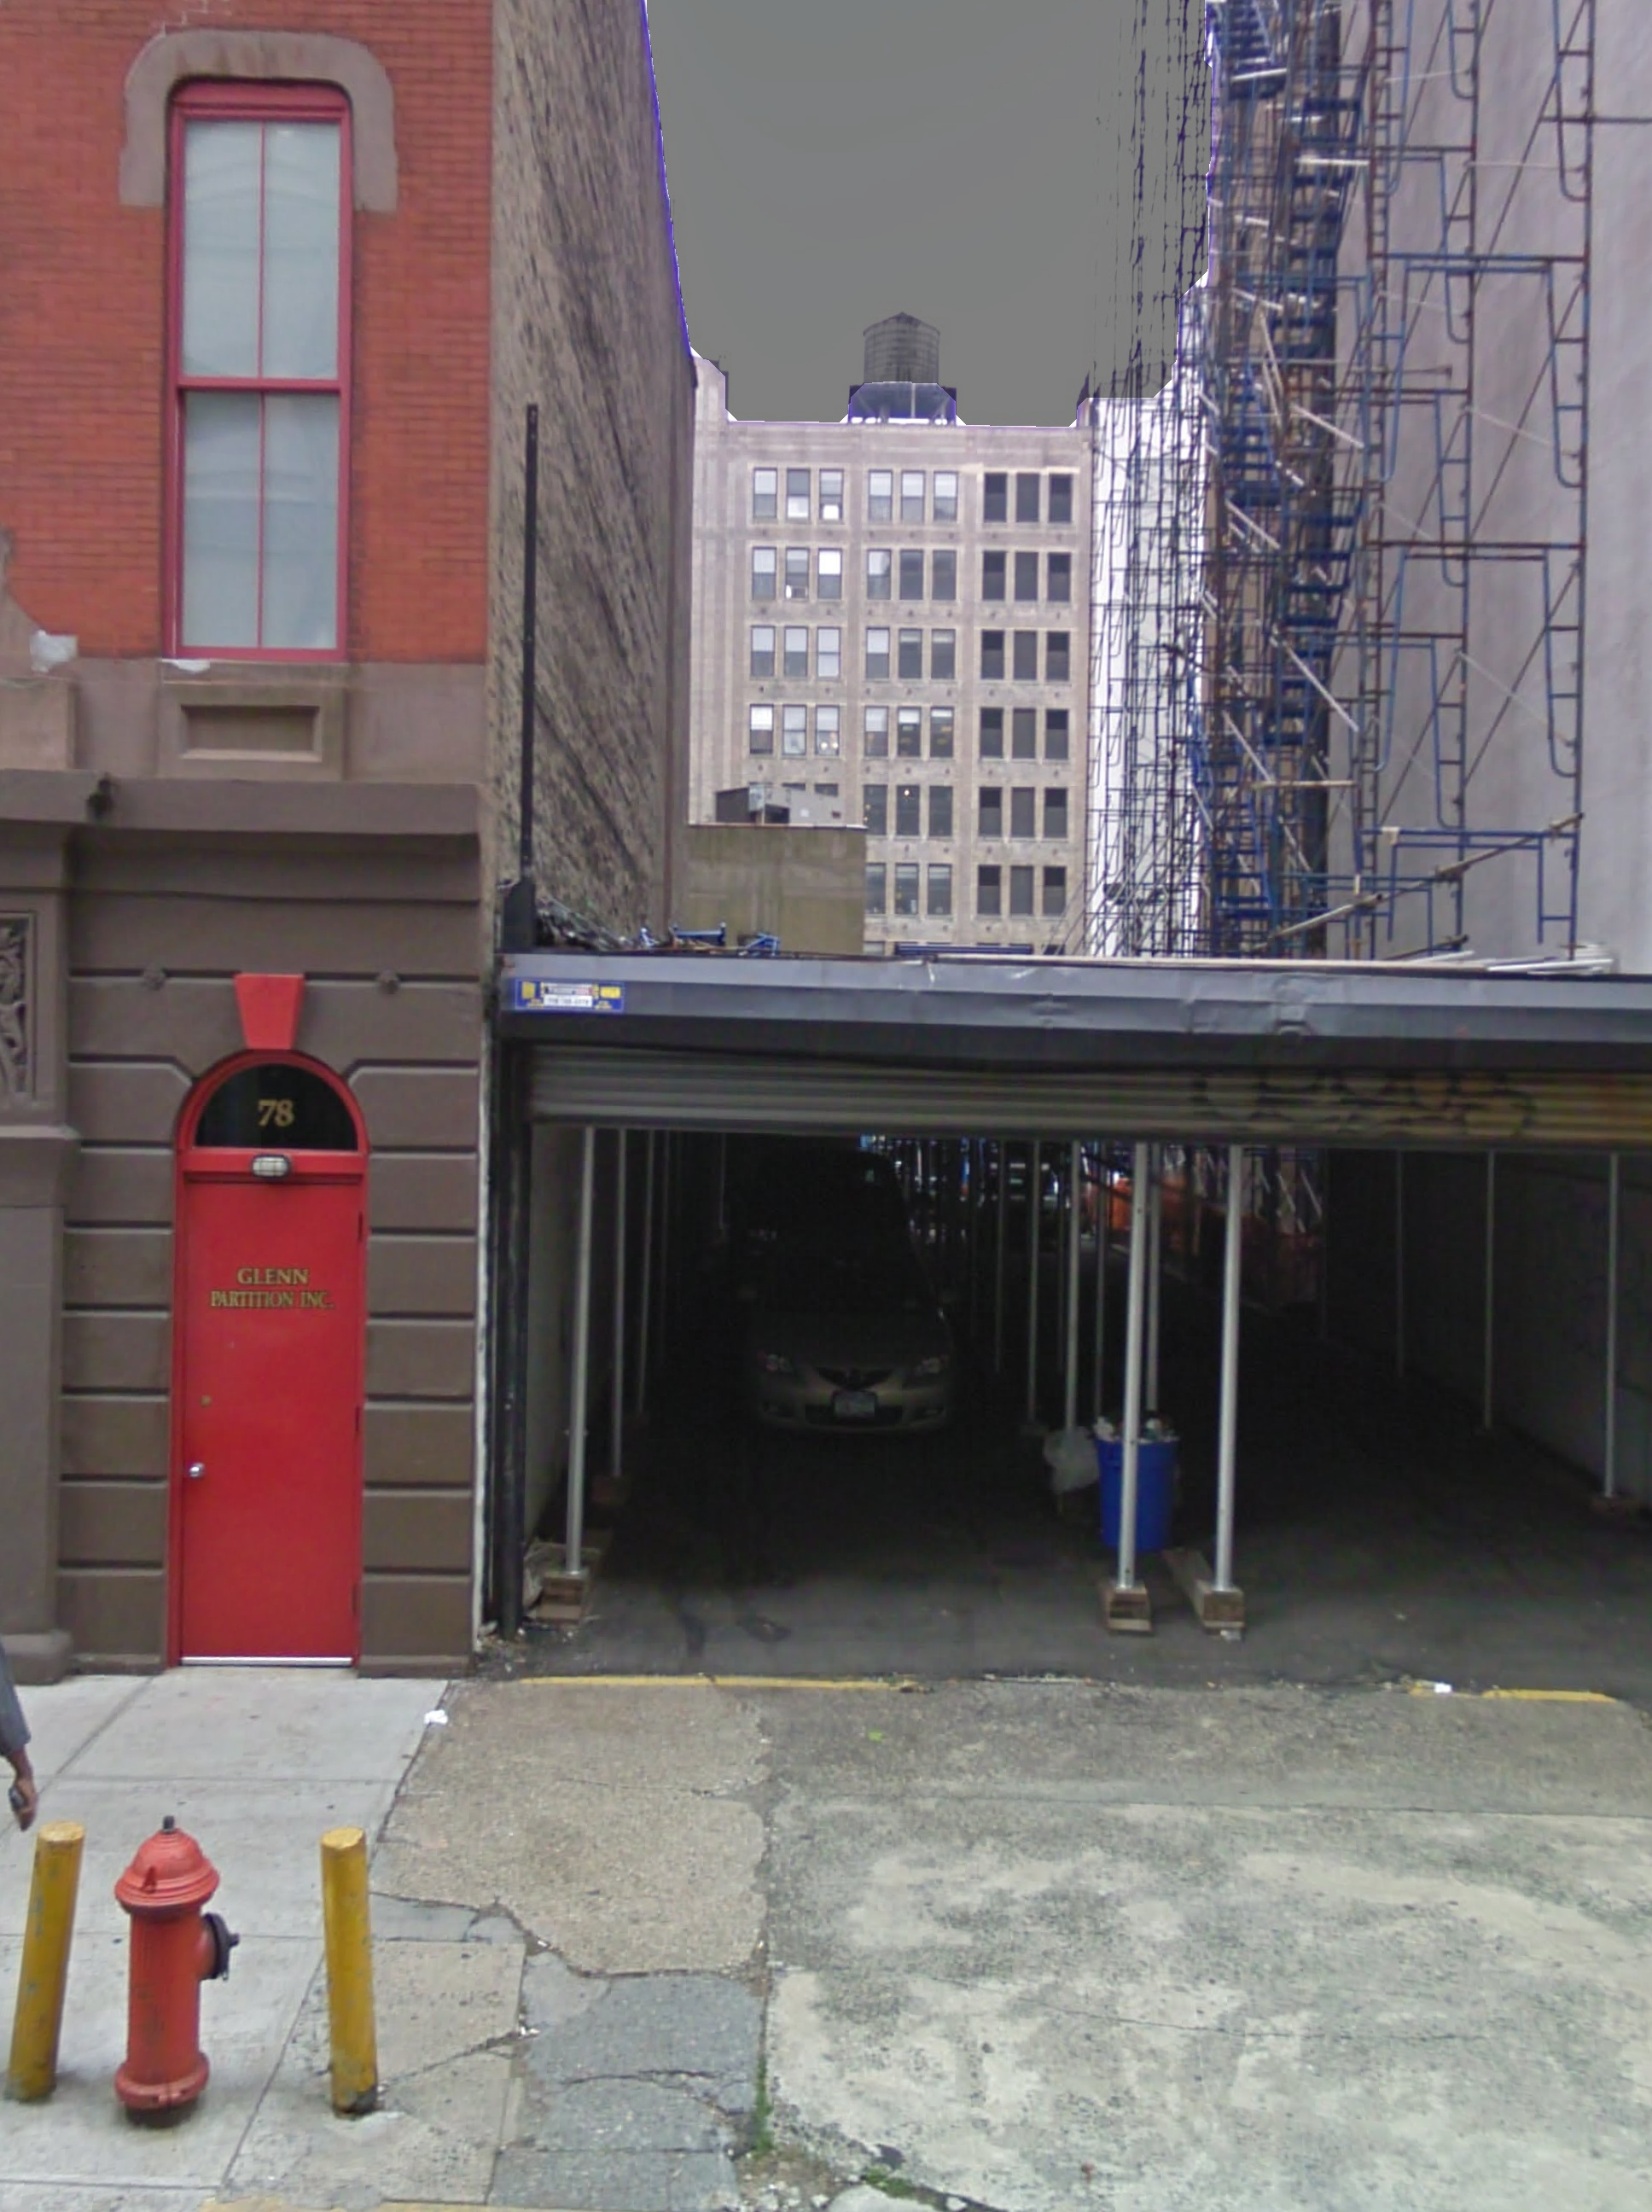
\includegraphics[height=0.3\linewidth]{./fig/overlay_02_02_ising.jpg}
}
\subfigure[LaserCut]{
\label{fig-lc_02_02}
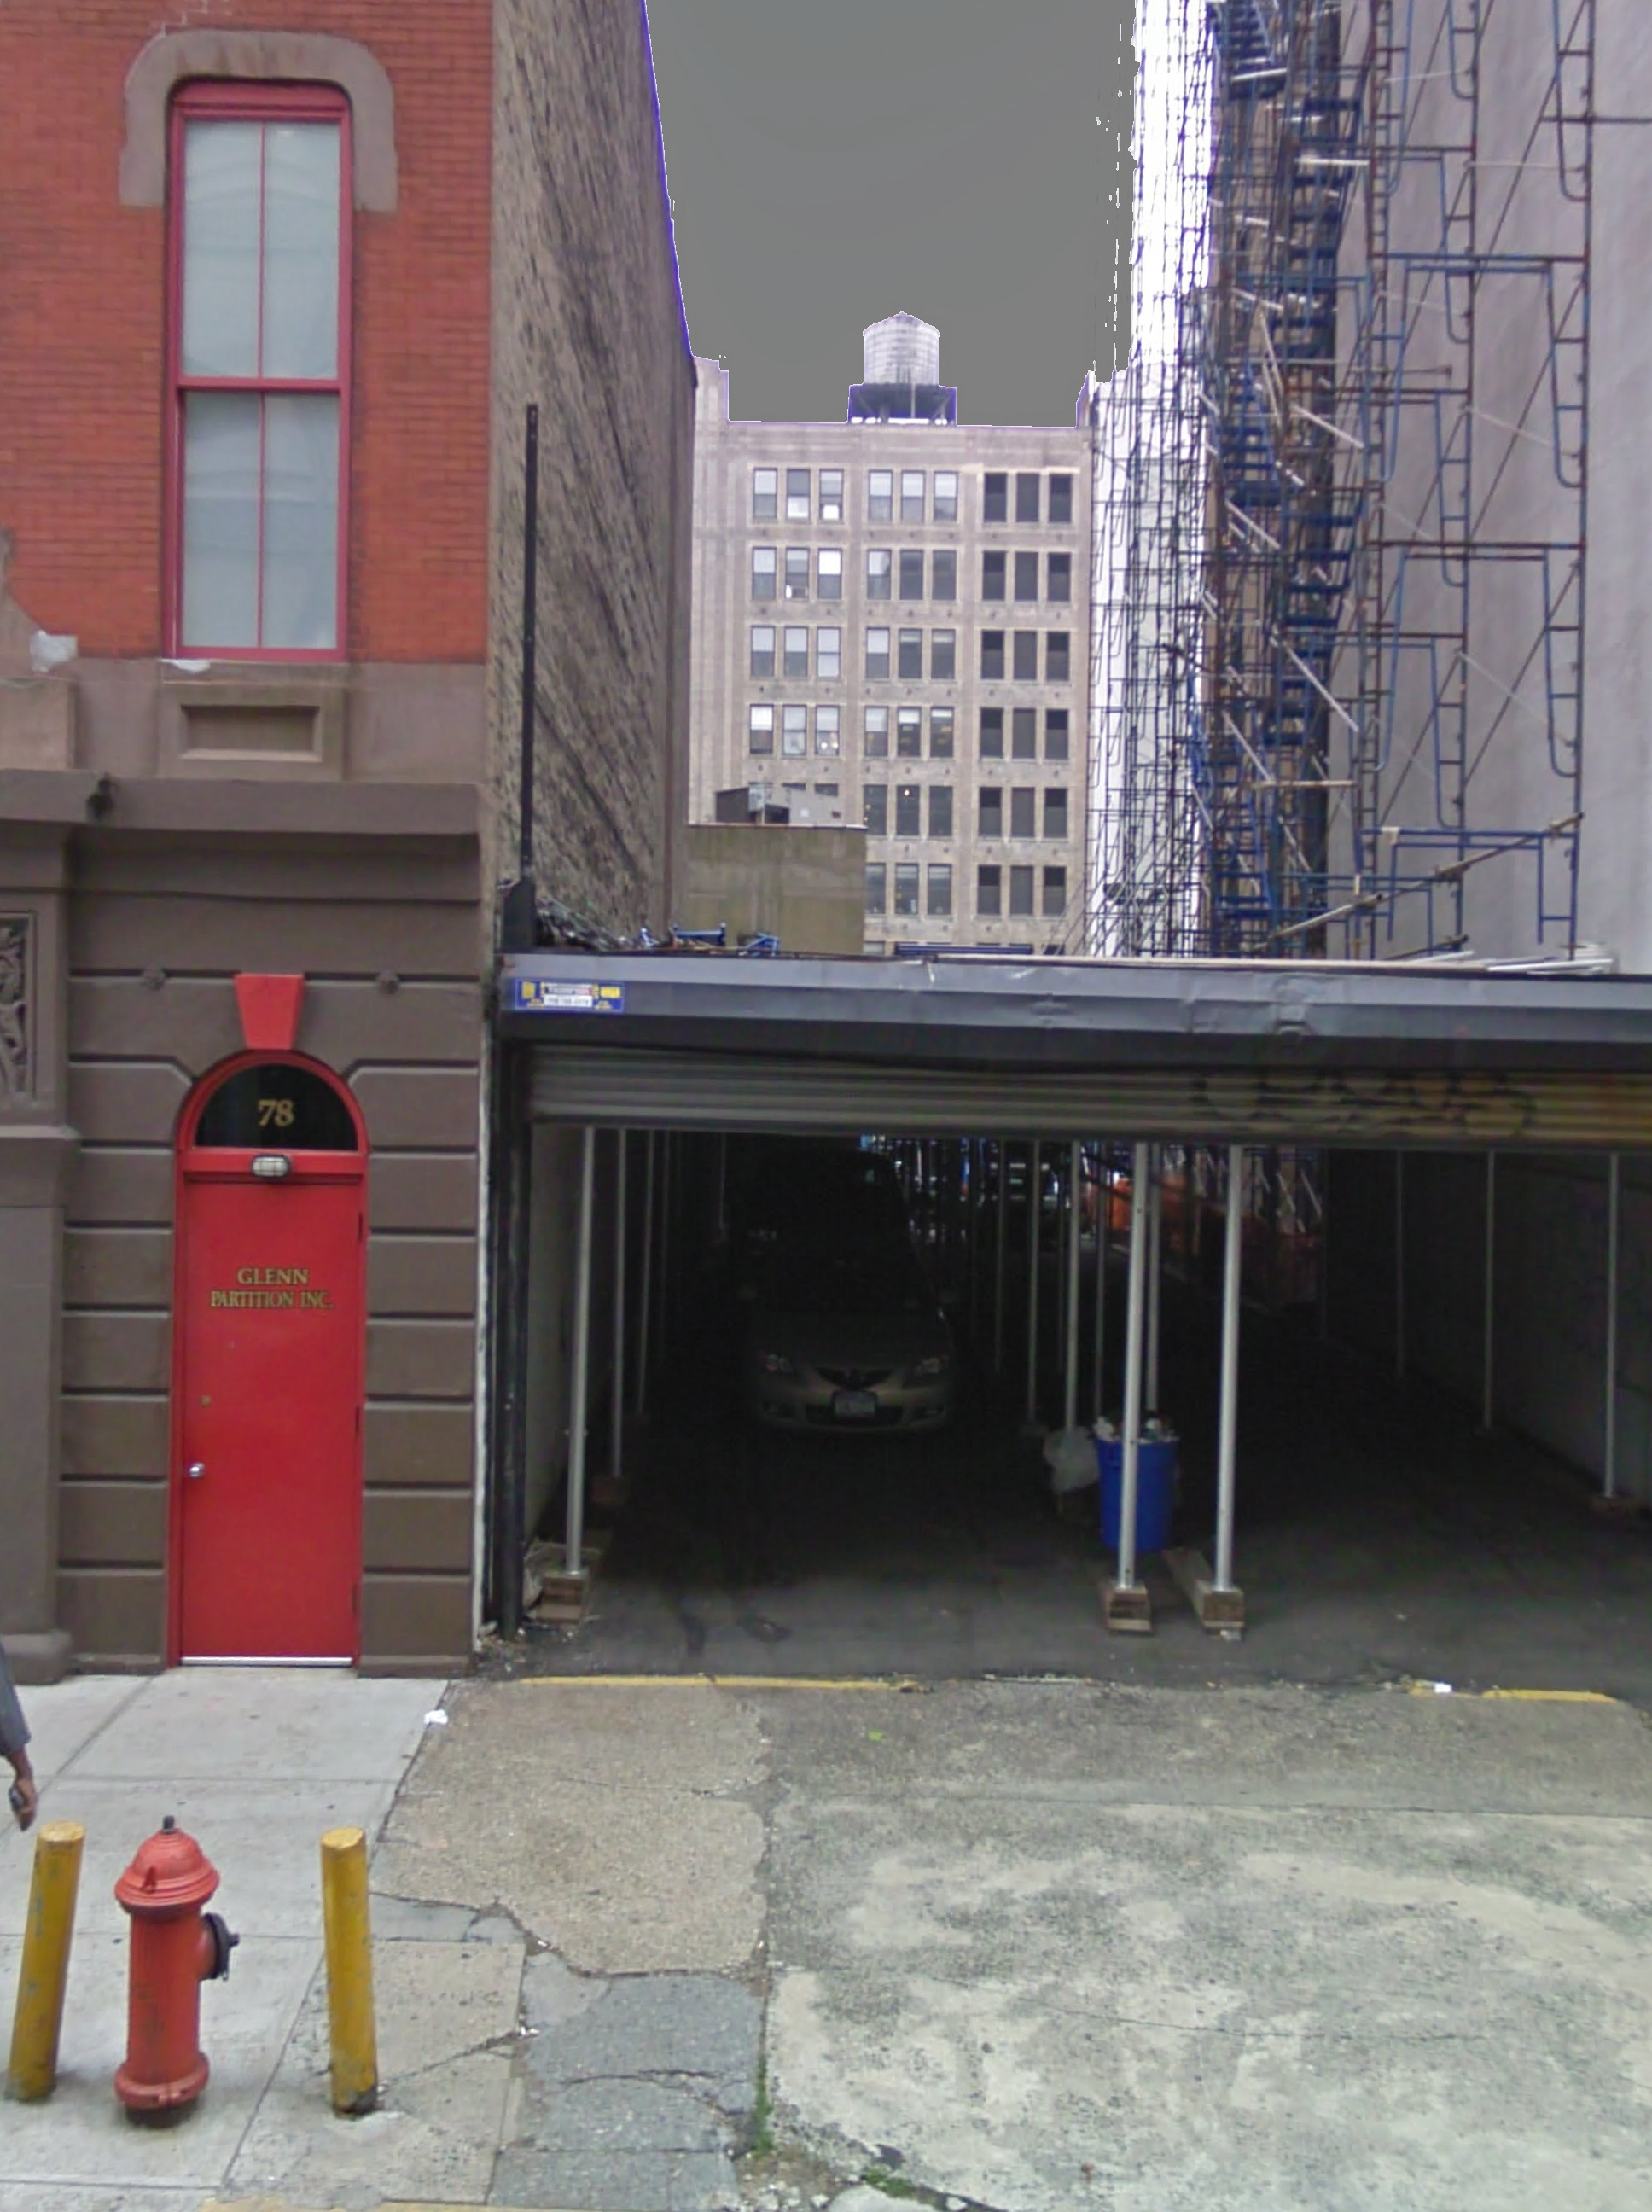
\includegraphics[height=0.3\linewidth]{./fig/overlay_02_02_laser.jpg}
}
\subfigure[Original image]{
\label{fig-im_14_04}
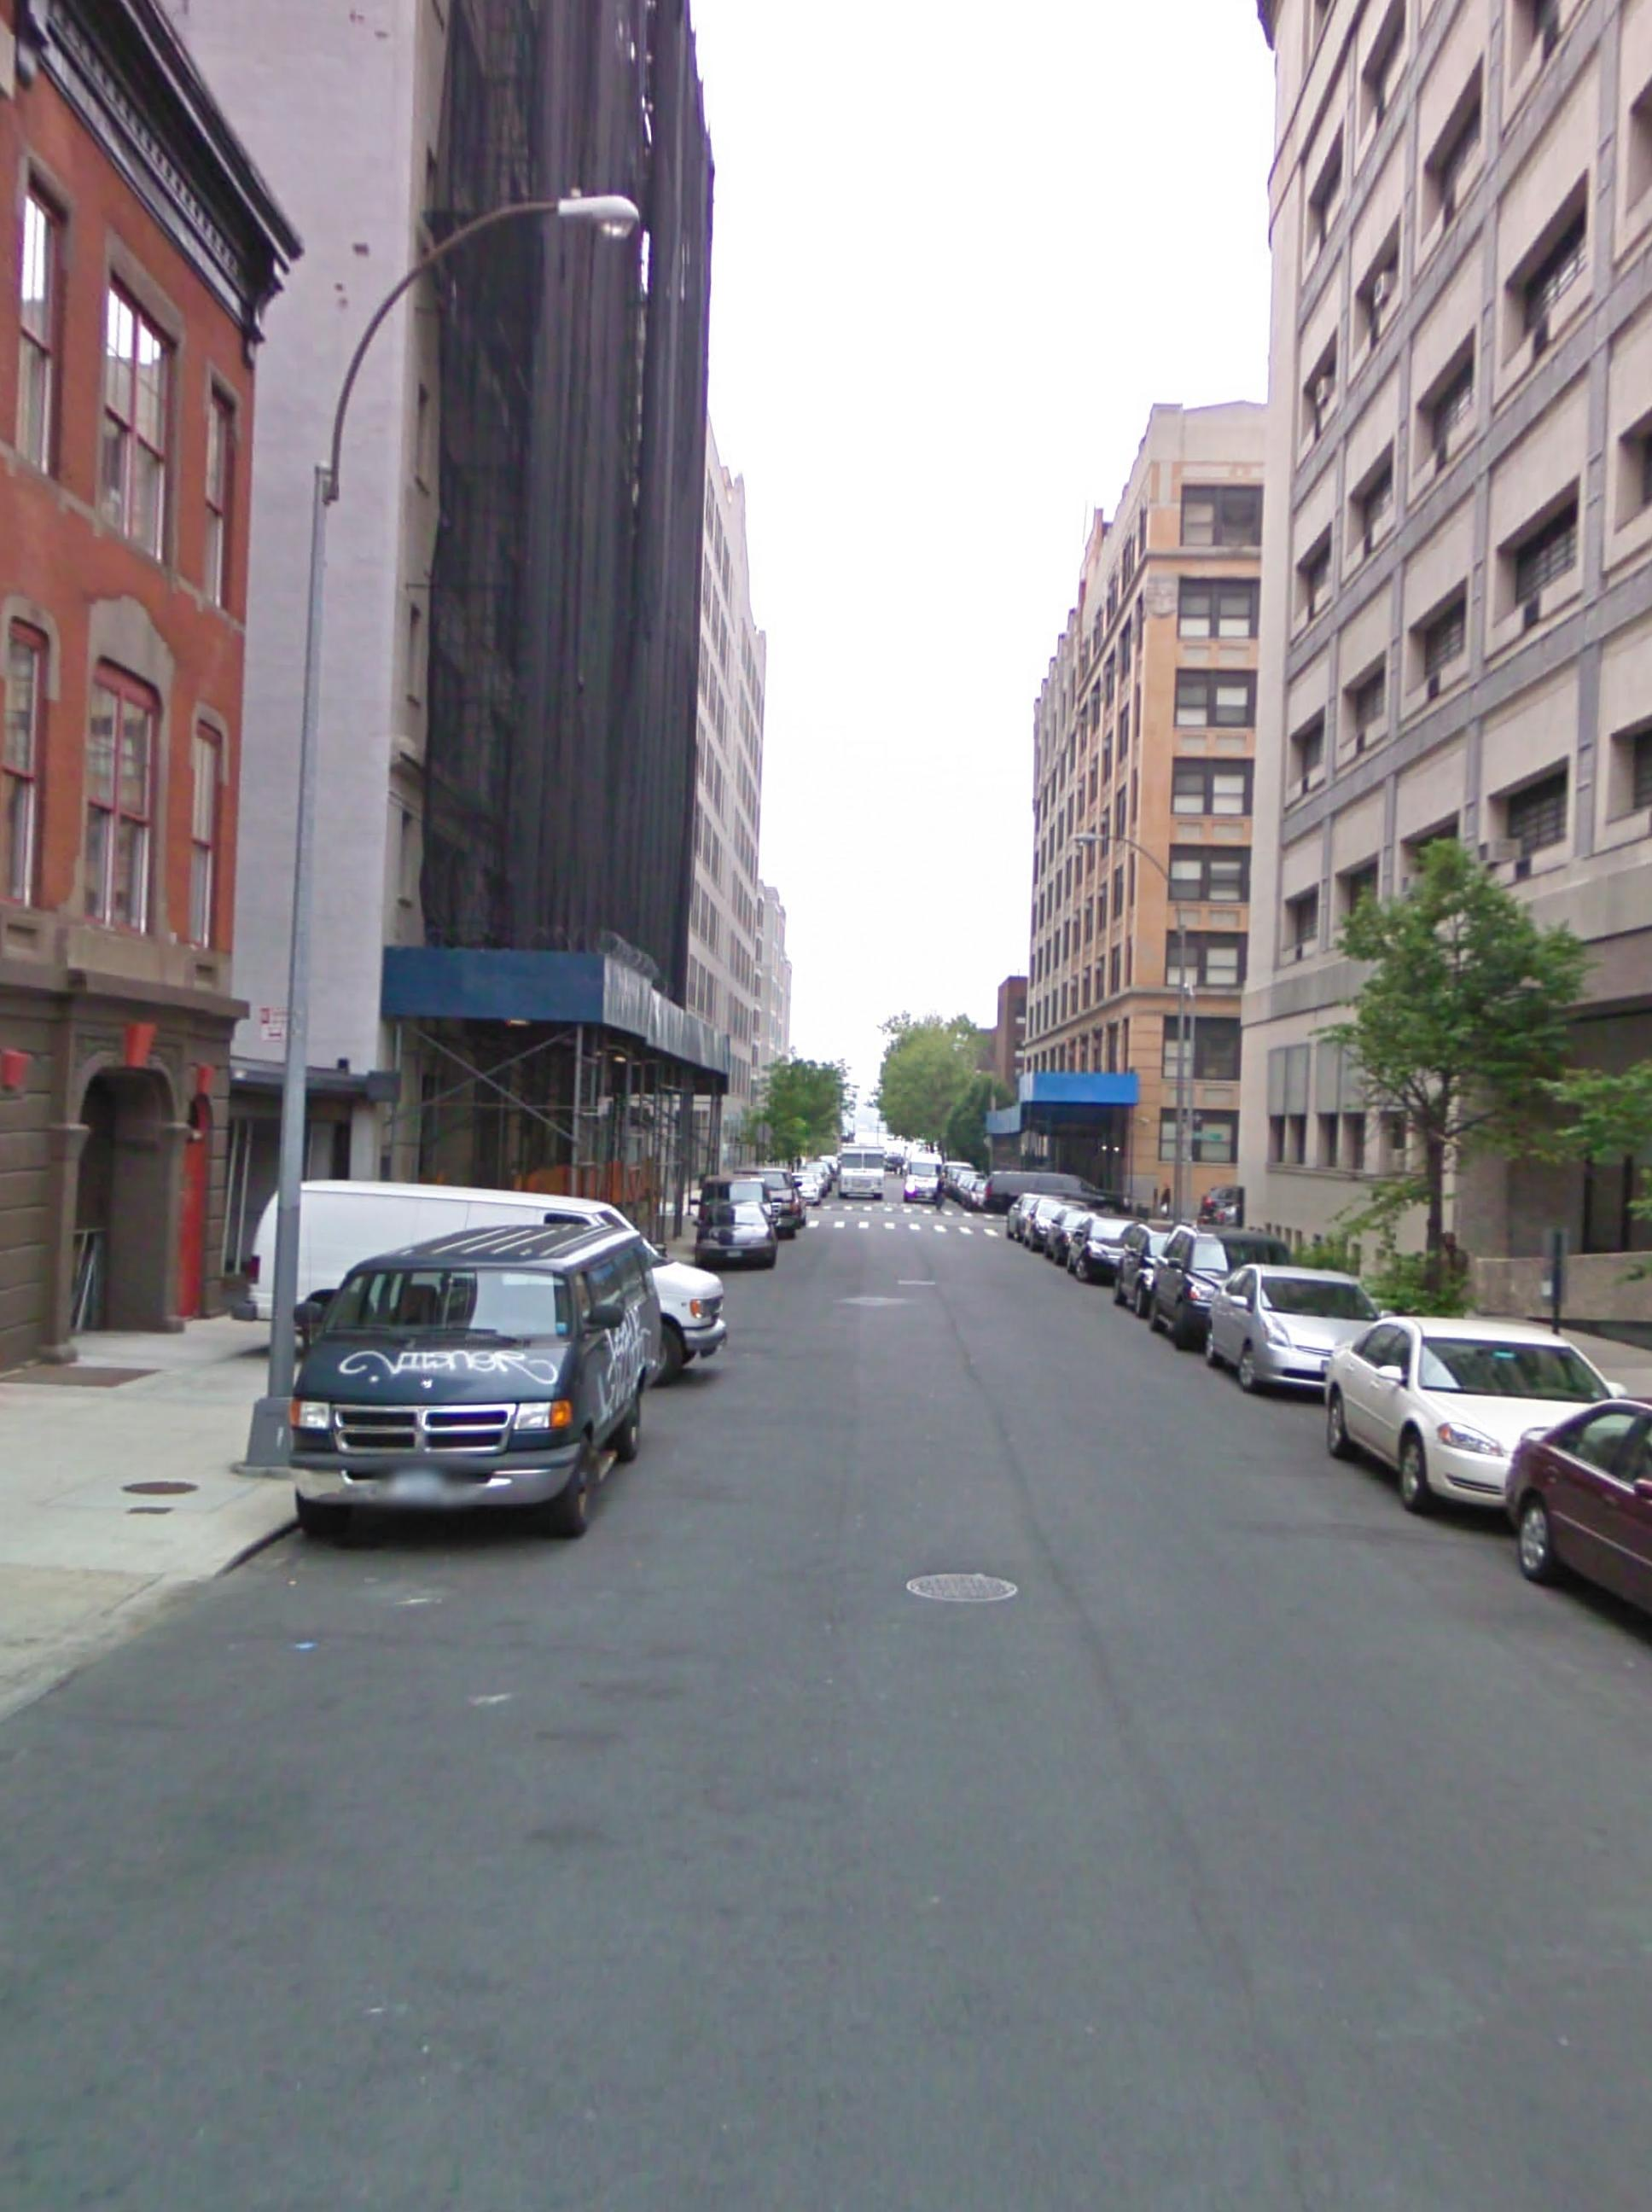
\includegraphics[height=0.3\linewidth]{./fig/image_14_04.jpg}
}
\subfigure[GrabCut]{
\label{fig-gc_14_04}
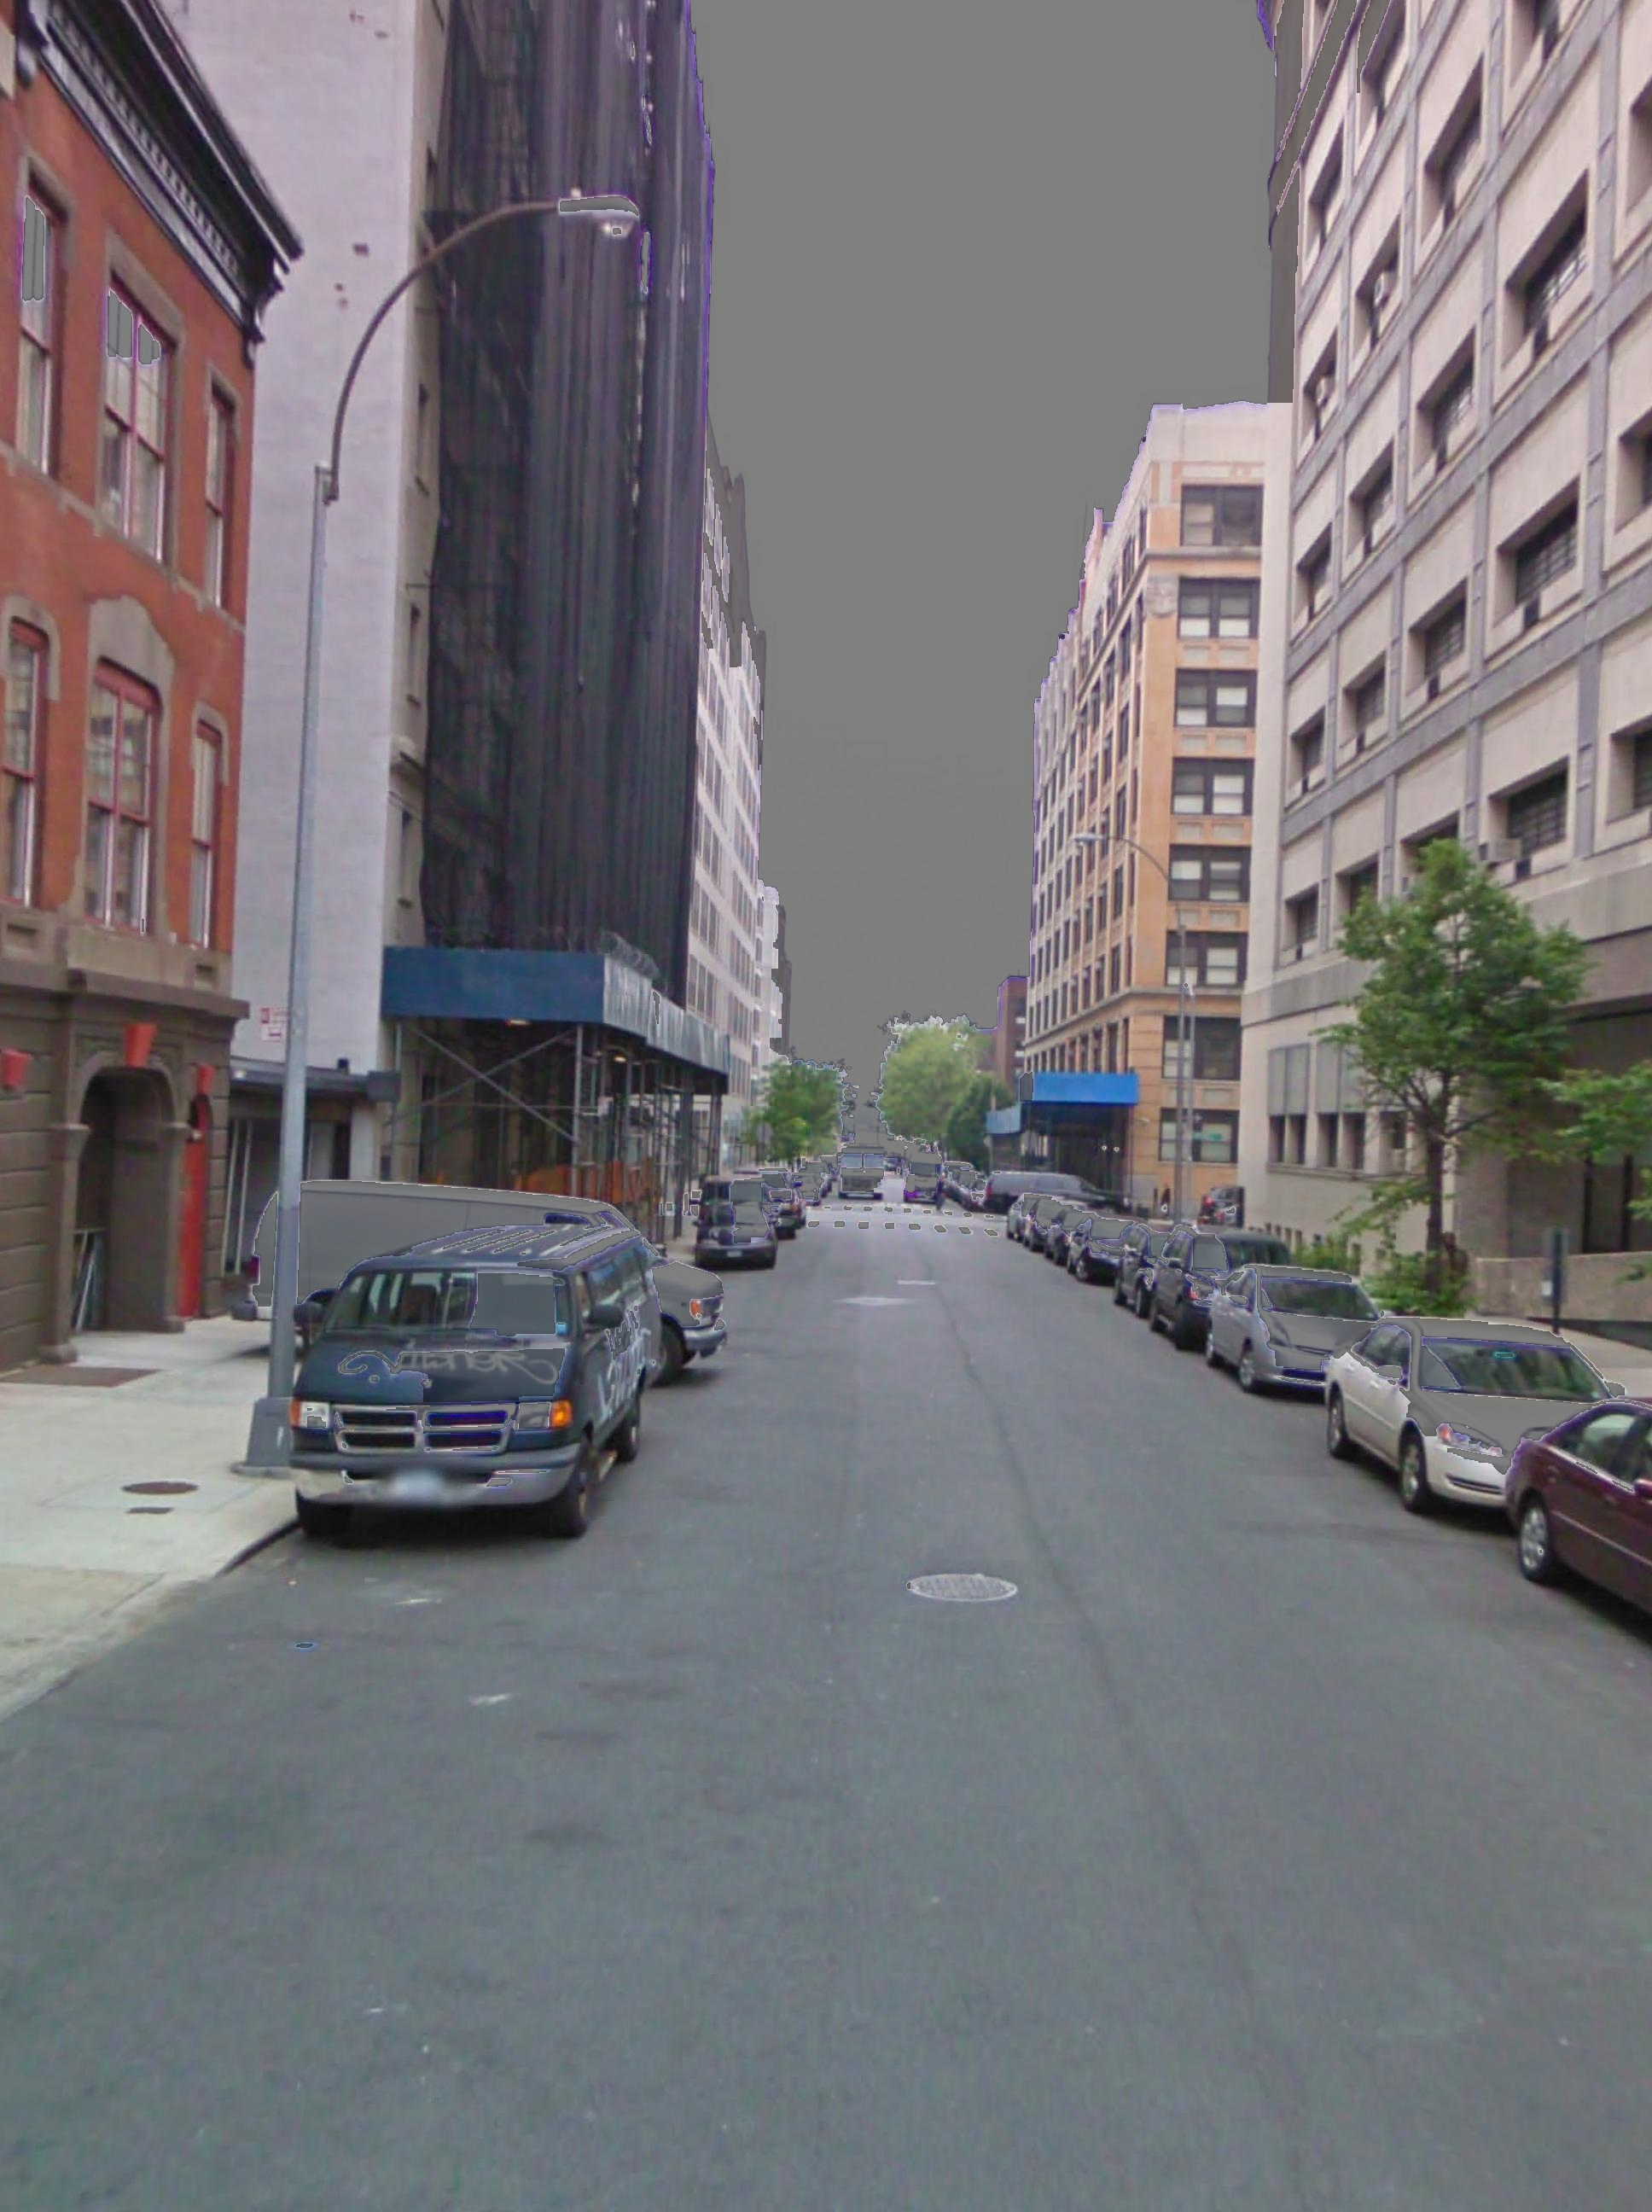
\includegraphics[height=0.3\linewidth]{./fig/overlay_14_04_grab.jpg}
}
\subfigure[Ising Model]{
\label{fig-is_14_04}
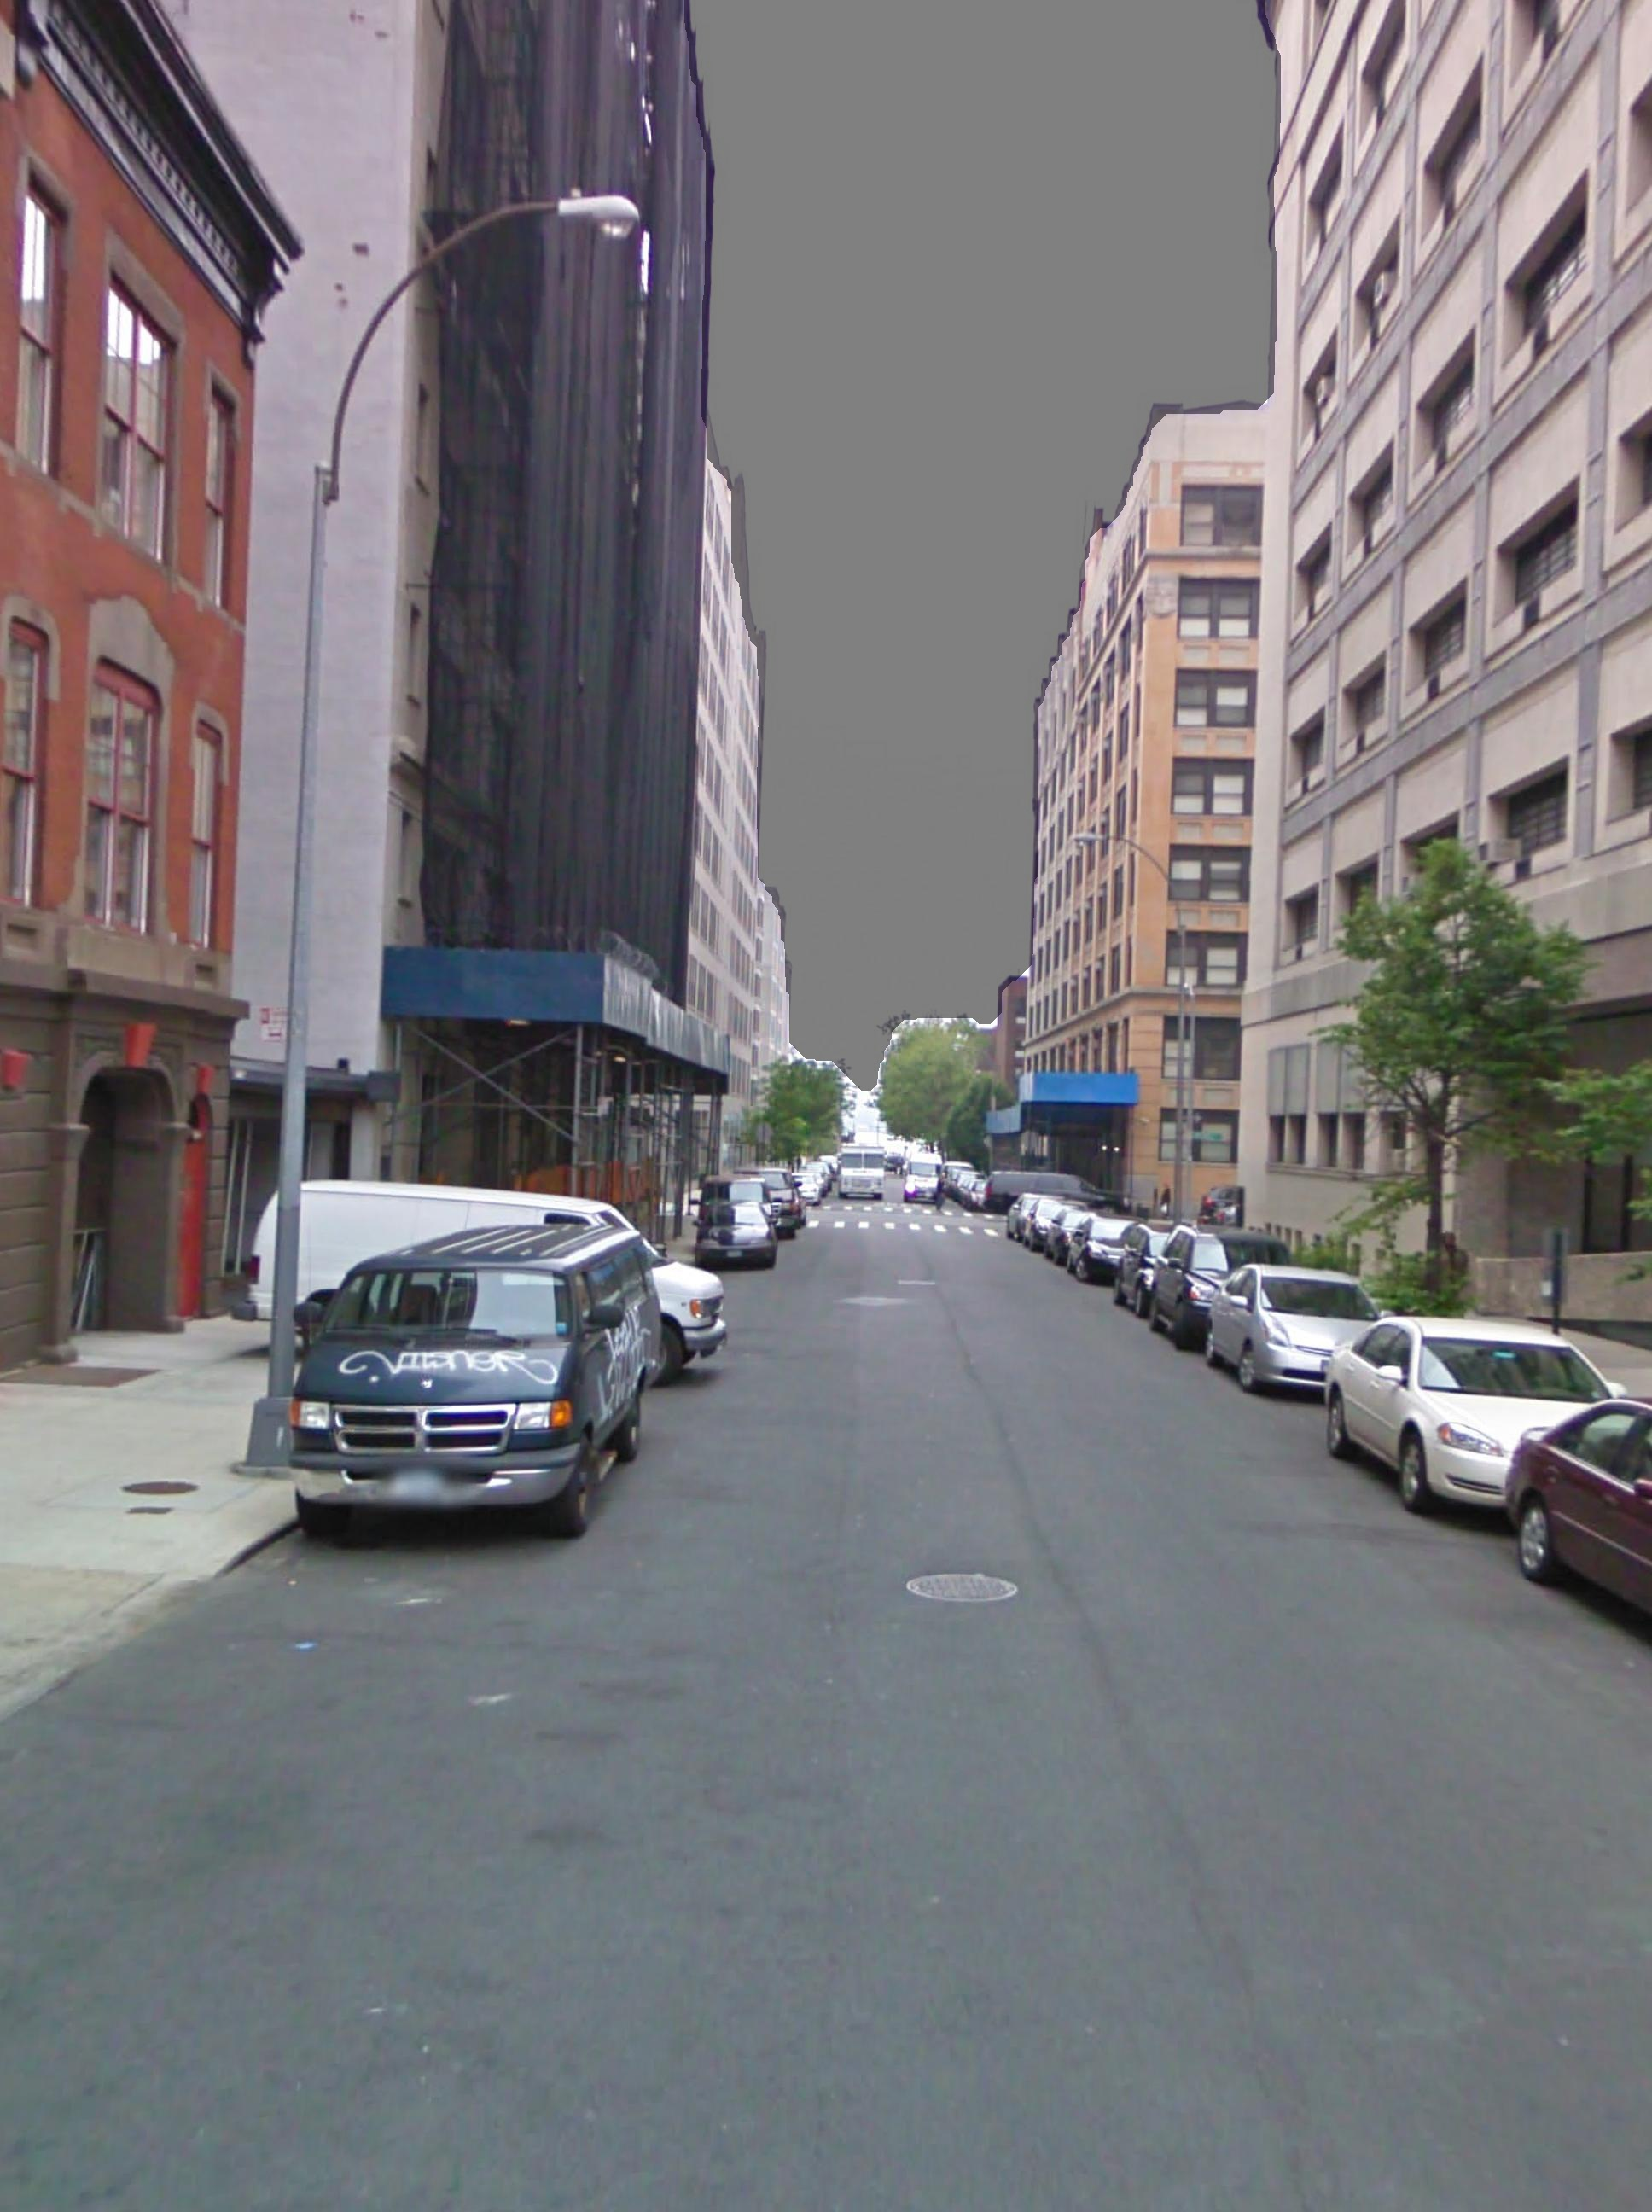
\includegraphics[height=0.3\linewidth]{./fig/overlay_14_04_ising.jpg}
}
\subfigure[LaserCut]{
\label{fig-lc_14_04}
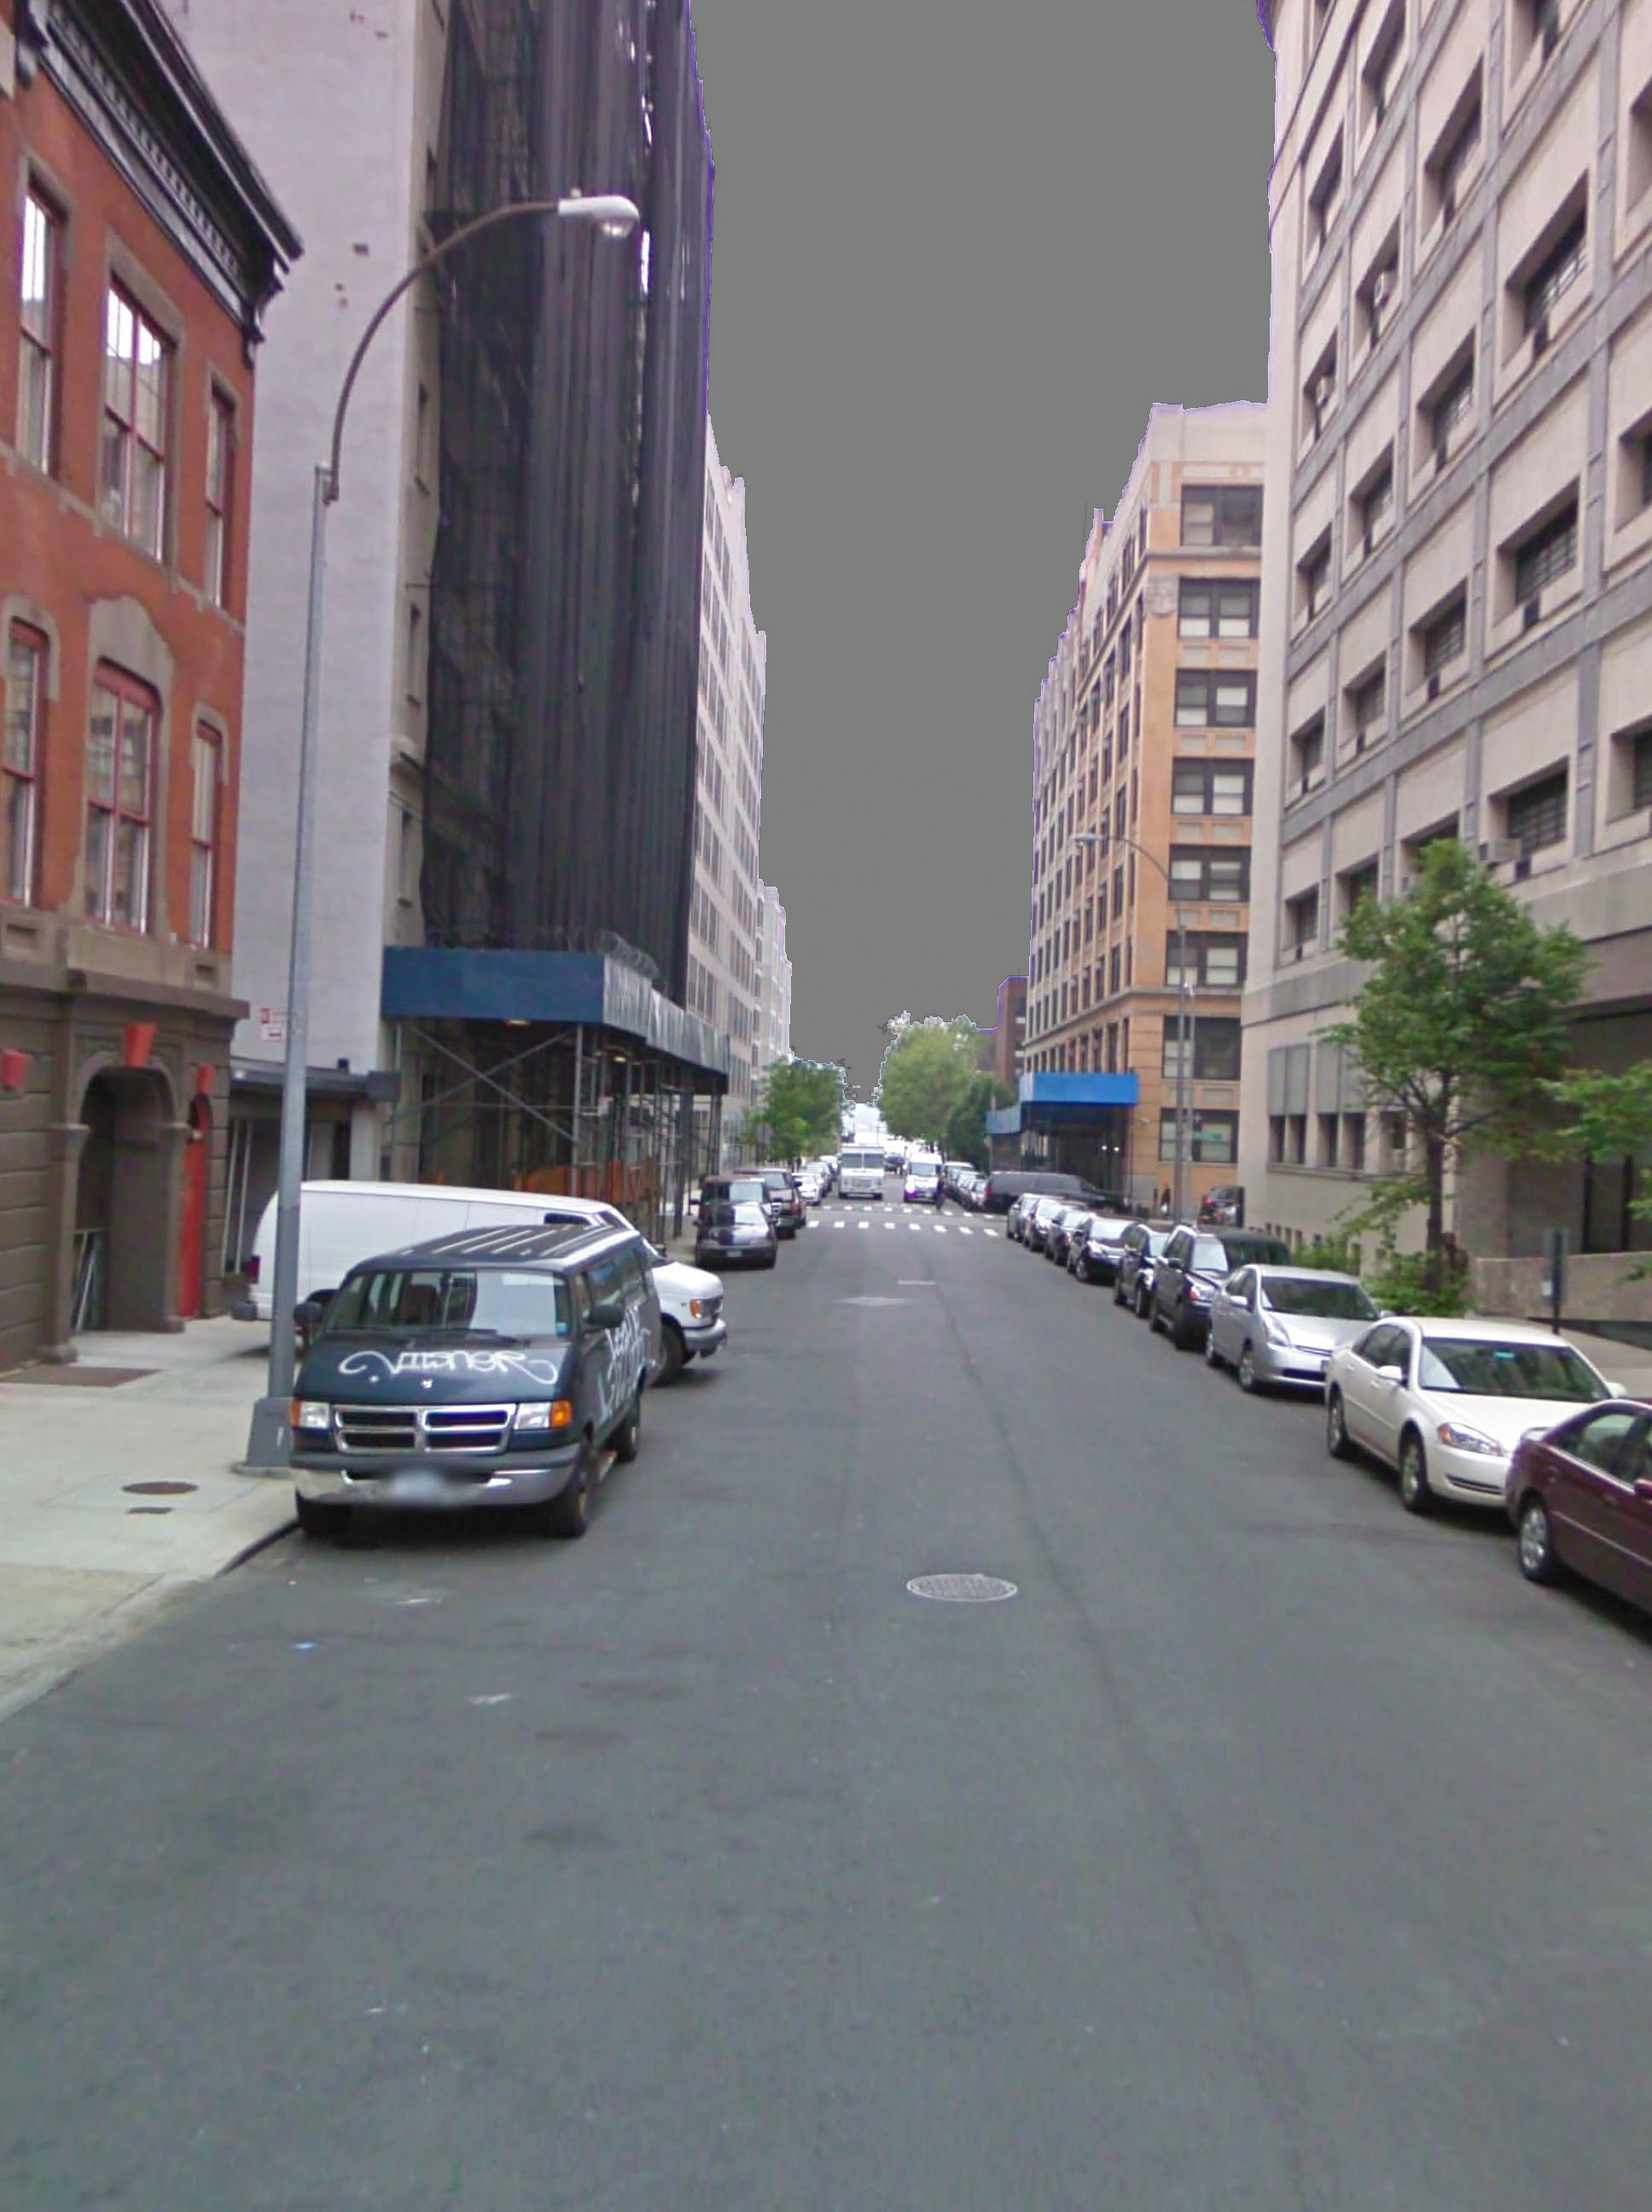
\includegraphics[height=0.3\linewidth]{./fig/overlay_14_04_laser.jpg}
}
\end{center}
\caption{Comparison study on other images.}
\label{fig-02_02}
\end{figure}

As we argued before, our algorithm would usually produce a more complicated yet cleaner bounary between forground and background over ther other two.

\bibliography{final}
\bibliographystyle{abbrvnat}


\end{document}
